
\section{Introduction}

The delocalization-localization transition for random operators has been a central question in probability theory and mathematical physics since the introduction of the Anderson model. Precisely, this model is a discrete random Schr\"{o}dinger operator on $\Z^{d}$ of the form $-\Delta+\lambda V$, where $\Delta$ is the graph Laplacian on $\Z^{d}$, where $V$ is a random potential with i.i.d. entries, and where $\lambda\in\R$. There has been a lot of work \cite{FroSpen_1985,Bourgain2005,Carmona1987,DingSmart2020,Damanik2002,Germinet2013,LiZhang2019} showing the existence of localized states, but the existence of delocalized states has been addressed in only one work \cite{yang2024Del} in high dimension, to our knowledge. 

A popular model \cite{PB_review,Spe} that has received a lot of attention and is conjectured to exhibit similar behavior to the random Schr\"{o}dinger operator is the $d$-dimensional \emph{random band matrix}. This is a random Hermitian matrix $H=(H_{xy})_{x,y}$ of dimension $N\times N$ whose entries are independent mean-zero complex random variables (up to the Hermitian constraint). The indices $x,y$ belong to the torus $(\Z/\sqrt[d]{N}\Z)^{d}$, and the variance profile $S_{xy}=\E|H_{xy}|^{2}$ vanishes if the distance between $x,y$ exceeds a band-width parameter $W$ depending on $N$.

In the case of dimension $d=1$, it was conjectured that \cite{PhysRevLett.64.1851, PhysRevLett.64.5, PhysRevLett.66.986} bulk eigenvector and eigenvalue statistics of $H$ match those of the \emph{Gaussian unitary ensemble} (GUE) if $W\gg N^{1/2}$. This was shown in \cite{YY_25} for Gaussian band matrices and a block variance profile. {The work \cite{YY_25} was also extended in \cite{ER_25_band} to non-Gaussian entries and more general variance profiles.} See also \cite{BaoErd2015, erdHos2013local, EK_band1,ErdKno2011, HeMa2018,bourgade2017universality, bourgade2019random,bourgade2020random,yang2021random,DY}, which place stronger assumptions on the band width $W$. On the other hand, it is conjectured that if $W \ll N^{1/2}$, the eigenvectors of $H$ are localized, which differs from GUE eigenvector statistics. This has been shown for a general class of band matrices in \cite{D_25}, building on previous results \cite{https://doi.org/10.48550/arxiv.2206.05545, https://doi.org/10.48550/arxiv.2206.06439,Sch2009,PelSchShaSod} under stronger assumptions on $W$.

The focus of this paper is dimension $d=2$. Random band matrices are expected to behave similarly to the Anderson model for $\lambda\sim W^{-1}$. Based on this connection and non-rigorous work \cite{PRL_Anderson} for the Anderson model, it is conjectured that bulk eigenvectors of $H$ are delocalized (and more generally that bulk eigenvalue and eigenvector statistics of $H$ match those of the GUE) when $W\gg\sqrt{\log N}$. See \cite{PB_review,Spencer1,Spencer2,Spencer3} for a further discussion.



The purpose of this paper is to establish a proof of the conjecture in dimension $d=2$, in the setting of complex Gaussian entries and under the slightly stronger assumption that $W \gg N^{\e}$ for some fixed $\e>0$. To explain this result, we recall the notion of the localization length of a band matrix ensemble, defined as the minimal scale $R$ such that the overwhelming majority of the mass of a typical bulk eigenvector is concentrated within a ball of radius $R$. In dimension $d=1$, \cite{YY_25} establishes delocalization at the conjectured threshold $W\gg\sqrt{N}$, so that the localization length reaches the conjectured scale $R \asymp W^2$. Our result in dimension $d=2$ implies that for any fixed $D$, one has $R \geq W^D$ provided $\mathfrak{c}$ is taken small enough. In comparison, all previous results established only $R \ge W^{1+c} $ for some $ c < 1$ in  dimension $d=2$ (see, e.g., \cite{ErdKno2011,EK_band1,erdos2013delocalization}). The precise model and the main results are presented in the next section.




Let us now briefly discuss some of the technical contributions of this paper. The analysis of band matrices in many of the aforementioned works is built on the following $T$-matrix associated to the band matrix $H$:
%
\begin{align*}
T_{ab}=\sum_{x}S_{ax}|G_{xb}|^{2}, \quad\text{where } S_{ax}:=\E|H_{ax}|^{2}.
\end{align*}
%
Above, $G:=(H-z)^{-1}$ denotes the resolvent of $H$ at a spectral parameter $z$ in the upper-half plane. In \cite{DY}, the analysis of the $T$-matrix was carried out by embedding $H$ inside a matrix Brownian motion and taking a time-dependent spectral parameter. This analysis was extended substantially in \cite{YY_25}, which recognized the importance of a more general hierarchy of dynamical ``loop" objects. These loops are essentially polynomials in the (now time-dependent) resolvent $G_{t}$; see \eqref{Eq:defGLoop} for the exact definition. 

Key to the analysis of the loop hierarchy in \cite{YY_25} for dimension $d=1$ is controlling quantities such as
%
\begin{align*}
\sum_{\textbf{b}}\mathcal{U}_{\textbf{a}\textbf{b}}\cdot\mathcal{P}(G_{t})_{\textbf{b}}.
\end{align*}
%
Above, the indices are $\textbf{a}=(a_{1},\ldots,a_{n})$ and $\textbf{b}=(b_{1},\ldots,b_{n})$ with $a_{i},b_{i}$ in the discrete torus. Also, $\mathcal{U}$ is a deterministic tensor with some smoothness properties in $\textbf{a},\textbf{b}$, and $\mathcal{P}(G_{t})_{\textbf{b}}$ is a polynomial in the entries of $G_{t}$ with indices close to those in $\textbf{b}$. In \cite{YY_25}, the control of such sums is done using the so-called ``sum-zero property", which ultimately lets one replace $\mathcal{U}$ with its discrete gradient and take advantage of its regularity. 

However, in $d=2$, the sum-zero property alone is insufficient to control these sums, because the number of terms in said sums is substantially larger than in $d=1$. This is one of the key challenges in $d=2$. 

\begin{comment} 
To resolve this issue, it suffices to show that the resolvent \(G=(H-z)^{-1}\) is \(\ell_z\)-dependent in the sense of an \(m\)-dependent random field. More precisely, as in the case \(d=1\), one first proves that the resolvent of a band matrix exhibits off–diagonal decay as in \eqref{Eq:Gdecay}, i.e.,
\[
\|x-y\|\gg \ell_z \ \Longrightarrow\  G_{xy}(z)\approx 0,\qquad x,y\in\mathbb Z_{\cor \sqrt N}^d .
\]
We then establish the \(\ell_z\)-dependence of \(G(z)\):
\[
\mathrm{dist}\!\big(\{x,y\},\{x',y'\}\big)\gg \ell_t \ \Longrightarrow\  G_{t,xy}\ \text{ and }\ G_{t,x'y'}\ \text{are almost independent}.
\]
This independence will be used in establishing the fluctuation cancellation effect mentioned above. This effect will be a key step in proving 
the quantum diffusion.  Without this cancellation,  errors would accumulate along the propagation. The phenomenon arises only for \(d\ge 2\) and it is a key ingredient in the analysis of  delocalization of band matrices in \(d\ge 3\) ~\cite{DYYY25}.
\end{comment} 

One of the novel contributions of this paper, which helps address this difficulty, is a set of new CLT-type estimates for $\mathcal{P}(G_{t})$. (That is, we control $\mathcal{P}(G_{t})_{\textbf{b}}$ in addition to using regularity of $\mathcal{U}$.) The proof of these estimates is based on carefully analyzing correlations between entries of $G_{t}$ in terms of the band width of the matrix $H$. This yields a new tool for the analysis of random band matrices, and the estimates themselves are perhaps of independent interest as well.

Let us illustrate the CLT-type estimates for the following simple example of $\mathcal{P}(G_{t})$, in which $\ell\gg1$ and $x$ is fixed:
%
\begin{align*}
\sum_{|y|\leq \ell} (G_{t})_{xy}.
\end{align*}
%
For $d=2$, the triangle inequality shows that this sum scales as $O(\ell^{2})$ with respect to $\ell$. In order to improve substantially on this, we will show cancellation between different $G_{t}$ entries in the above sum and obtain an estimate of $O(\ell\cdot\ell_{t})$ in dimension $d=2$. Here, $\ell_{t}\ll\ell$ is a dynamical length-scale that captures the correlation length of $G_{t}$ entries. 



Roughly speaking, we will prove in  $d=2$ that there is a scale $\ell_t$ such that 
\[
\|x-y\|\gg \ell_t \ \Longrightarrow\  G_{t, xy}\approx 0,\qquad x,y\in\mathbb Z_{WL}^{2} .
\]
We then show   the \(\ell_t\)-independence of \(G_{t}\), i.e., 
\[
\mathrm{dist}\!\big(\{x,y\},\{x',y'\}\big)\gg \ell_t \ \Longrightarrow\  G_{t,xy}\ \text{ and }\ G_{t,x'y'}\ \text{are almost independent}.
\]
This independence will be used in establishing the fluctuation cancellation mentioned above. This effect will be a key step in proving 
the quantum diffusion.  Without this cancellation,  errors would have accumulated along the time evolution. This  phenomenon arises only for 
\(d\ge 2\) and it is  a key ingredient in the proof  of  delocalization of band matrices in \(d\ge 3\) ~\cite{DYYY25}.


%This property guarantees the stability of quantum diffusion; otherwise, errors would accumulate along the time evolution. The phenomenon arises only for \(d\ge 2\), since in this regime the diffusion volume is of order \(\ell_z^{\,d}\), which is much larger than the single–edge scale \(\ell_z\). Consequently, \(\ell_z\)-dependence is a key ingredient for other high–dimensional non–mean–field models as well. It also enters as a central input in the \(d\ge 3\) delocalization proof~\cite{DYYY25} and in the analysis of the block Anderson model~\cite{RBSO1D}.





We conclude this introduction with a discussion of related results. The proof of the full delocalized phase, quantum diffusion, and universality of local eigenvalue statistics for dimension $d\geq 7$ was shown in \cite{yang2021delocalization, yang2022delocalization, Xu:2024aa}, which uses an expansion method for the resolvent of $H$. In dimension $d=3$, for special variance profiles of $H$, supersymmetric methods have been used \cite{DisPinSpe2002} to estimate the density of states for $H$. Similar methods have also been able to detect the transition between $W\gg N^{1/2}$ and $W\ll N^{1/2}$ at the level of two-point functions in $d=1$ \cite{Shcherbina:2021wz}. See \cite{BaoErd2015, SchMT, Sch1, Sch2, Efe1997, Spe} for further discussion on the supersymmetric method.


\subsection*{Acknowledgements}
K.Y. was supported in part by NSF Grant No. DMS-2203075.




\section{The model and main results}\label{sec_model-results}
 \subsection{Band matrix model}\label{subsec_setting}

We will study the following two-dimensional band block matrix model. Fix positive integers $W>0$ and $L\geq3$, and set $N:=W^{2}L^{2}$. Let $\Z_{L}:=\Z/L\Z\simeq\{1,\ldots,L\}$.

The matrix of interest is $H=(H_{xy})_{x,y\in \Z_{WL}^{2}}$, where $H_{xy}=\overline{H}_{yx}$, and up to this Hermitian constraint, the entries $H_{xy}\sim\mathcal{CN}(0,S_{xy})$ are independent centered complex Gaussian random variables of variance $\E|H_{xy}|^{2}=S_{xy}$, where $S=(S_{xy})_{x,y\in \Z_{WL}^{2}}$ is a matrix with the following block structure. We define
%
\begin{align*}
S^{(B)}_{ab}&=\frac{1}{5}\mathbf{1}(|a-b|_{L}\leq1),\quad(S_{W})_{ij}=W^{-2},\quad a,b\in\Z_{L}^{2}, \ i,j\in\{1,\ldots,W\}^{2}.
\end{align*}
%
Note that $S^{(B)}$ is $L^{2}\times L^{2}$, and that $S_{W}$ is $W^{2}\times W^{2}$. Above, $|a-b|_{L}$ is the periodic $L^{1}$ distance on $\Z_{L}^{2}$. The standing assumption $L\geq3$ costs nothing, since all of our results are asymptotic as $N\to\infty$ and hence as $L\to\infty$; we record it because the displayed formula for $S^{(B)}$ does require it. For $L\leq2$ the five residues $0,\pm e_{1},\pm e_{2}$ of $\Z_{L}^{2}$ are not distinct, so the row sums of $S^{(B)}$ are $1/5$ when $L=1$ and $3/5$ when $L=2$, and $S^{(B)}$ is not stochastic. We now define $S$ to be the following real-symmetric, stochastic matrix:
%
\begin{align*}
S=S^{(B)}\otimes S_{W}.
\end{align*}
%
Note that the entries of $H$ and $S$ are indexed by $\Z_{WL}^{2}$. 

We now introduce standard notation for the setting of this paper. We start by letting $\lambda_{1}\leq\ldots\leq\lambda_{N}$ be eigenvalues of $H$ with corresponding unit eigenvectors $\boldsymbol{\psi}_{1},\ldots,\boldsymbol{\psi}_{N}$, so that
$$H\boldsymbol{\psi}_{k}=\lambda_{k}\boldsymbol{\psi}_{k}.$$ Our analysis of these quantities is based on the resolvent $G(z):=(H-z)^{-1}$ of $H$ defined for any $z$ with $\im z>0$. 

It is well known that the empirical spectral measure of $H$ converges almost surely to the Wigner semicircle distribution as $N\to\infty$ if $W\to\infty$. The Stieltjes transform of the semicircle distribution is given by
%
\begin{align*}
m(z):=\int_{-2}^{2}\frac{1}{2\pi}\frac{\sqrt{(4-x^{2})_{+}}}{x-z}dx=\frac{-z+\sqrt{z^{2}-4}}{2}.
\end{align*}
%
Finally, we will use a standard notion of stochastic domination as used in \cite{Average_fluc}, defined below.
\begin{definition}\label{stoch_domination}
	{\rm{(i)}} Consider the following two families of non-negative random variables parameterized by a set $U^{(N)}$:
	\[\xi=\left(\xi^{(N)}(u):N\in\mathbb N, u\in U^{(N)}\right),\hskip 10pt \zeta=\left(\zeta^{(N)}(u):N\in\mathbb N, u\in U^{(N)}\right).\]
	We say that $\xi$ is stochastically dominated by $\zeta$ (uniformly in $u$) if for any fixed (small) $\tau>0$ and (large) $D>0$, we have the following for $N\geq N_{0}(\tau,D)$:
	\[\mathbb P\bigg(\bigcup_{u\in U^{(N)}}\left\{\xi^{(N)}(u)>N^\tau\zeta^{(N)}(u)\right\}\bigg)\le N^{-D}\]
	We will use the notation $\xi\prec\zeta$ or $\xi=\mathrm{O}_{\prec}(\zeta)$ to mean that $\xi$ is stochastically dominated by $\zeta$. If $\xi$ is a family of complex numbers, then $\xi\prec\zeta$ and $\xi=\mathrm{O}_{\prec}(\zeta)$ mean that $|\xi|\prec\zeta$. 
	
	\vspace{5pt}
	\noindent {\rm{(ii)}} As a convention, for deterministic $\xi,\zeta\geq0$, we write $\xi\prec\zeta$ if and only if $\xi\le N^\tau \zeta$ for any fixed $\tau>0$. 

 \vspace{5pt}
	\noindent {\rm{(iii)}} Let $A$ be a family of random matrices and $\zeta$ be a family of non-negative random variables. In this case, we use $A=\OO_\prec(\zeta)$ to mean that $\|A\|\prec \zeta$, where $\|\cdot\|$ is the operator norm. 
	
	\vspace{5pt}
	\noindent {\rm{(iv)}} We say that an event $\Xi$ holds with high probability (w.h.p.) if for any $D>0$, we have $\mathbb P(\Xi)\ge 1- N^{-D}$ for large enough $N$. We say that an event $\Omega$ holds $w.h.p.$ in $\Xi$ if for any $D>0$, we have
	$\P( \Xi\setminus \Omega)\le N^{-D}$ for large enough $N$.
	%\end{itemize}
\end{definition}






\subsection{Main results}

Our first result states a strong delocalization estimate for bulk eigenvectors of $H$. 


\begin{theorem}[Delocalization]\label{MR:decol}
Suppose that the following is satisfied for some fixed constant $ \mathfrak c>0$: 
\begin{equation}\label{Main_DEL_COND}
    W \ge N^{\mathfrak c}. 
\end{equation}
Then for any $\kappa, \tau, D>0$, there exists $N_0$ such that for all $N \geqslant N_0$ we have
$$
\mathbb{P}\left( \max_k\left\|\boldsymbol{\psi}_k\right\|_{\infty}^2 \cdot {\bf1}\big(\lambda_k\in[-2+\kappa,2-\kappa]\big)\leqslant N^{-1+\tau}  \right) \geqslant 1-N^{-D}
$$
\end{theorem}

The proof of Theorem \ref{MR:decol} is based on estimates for the Green's function $G(z)$, which we state below. First, however, we need some more notation. We start with a ``diffusive" length-scale with respect to a parameter $z$ in the upper half plane:
%
\begin{align}
\ell:=\ell(z):=\min\left(\eta^{-1/2},L\right)+1, \quad\eta:=\im(z).\label{def_ellz}
\end{align}
%
We will also introduce the fundamental control parameter to be
%
\begin{align}
M_{\eta}:=W^{2}\ell(z)^{2}\eta,\quad\eta=\im(z).\label{def_meta}
\end{align}
%
Next, we introduce the following index set given any $a=(a(1),a(2))\in\Z_{L}^{2}$:
%
\begin{align*}
{\cal I}^{(2)}_{a}:={\cal I}_{a(1)}\times{\cal I}_{a(2)},\quad{\cal I}_{a(i)} := \left[ (a(i)-1)W + 1, \; a(i)W \right].
\end{align*}
%
\begin{theorem}[Local semicircle law]\label{MR:locSC} Suppose that the assumption of Theorem \ref{MR:decol} holds. For any fixed $\kappa, \tau,D>0$, and for any $z\in\C$ of the form 
$$z=E+i\eta,\quad\quad |E|\le  2-\kappa, \quad 1\ge \eta\ge N^{-1+\tau},
$$
there exists $N_0$ such that for all $N \geqslant N_0$ we have the following estimates. First, we have the local law:
\begin{equation}\label{G_bound}
   \mathbb P\left( \max_{x,y}  \left|\left(G(z)-m(z)\right)_{xy}\right|\le  \frac{W^\tau}{\sqrt{M_{\eta}}}\right)\geqslant 1-N^{-D},\quad \ell=\ell(z).
\end{equation}
Second, we have the partial tracial local law
\begin{equation}\label{G_bound_ave}
\mathbb{P}\left(\max_a\Big| W^{-2}\sum_{x\in {\cal I}^{(2)}_a}G_{xx}(z)-m(z) \Big| \le \frac{W^\tau}{M_{\eta}} \right)\geqslant 1-N^{-D},\quad \ell=\ell(z). 
\end{equation}

\end{theorem}


We now state our next two results. The first of these is {quantum unique ergodicity}, and the second is a quantum diffusion profile for the resolvent. 
\begin{theorem}[Generalized quantum unique ergodicity]\label{MR:QUE} 
Suppose the assumptions of Theorem \ref{MR:decol} hold and 
\begin{align}\label{tau} 
0< \tau <  \frac {  \mathfrak c } 2, 
\end{align} 
where $ \mathfrak c$ was defined in \eqref{Main_DEL_COND}. Next, let $E_a$ denote the following  block identity matrix: 
\begin{equation}\label{Def_matE}
(E_a)_{xy}=  \delta_{xy}\cdot W^{-2}\cdot\textbf{1}(x\in {\cal I}^{(2)}_a),\quad x,y\in \Z_{WL}^{2}.
\end{equation}
Then  for any $\kappa>0$,
there exists   $N_0$ such that for all $N \geqslant N_0$, we have
\begin{equation}\label{Meq:QUE}
\max_{E: \,|E|<2-\kappa}\; 
\max_{ a\,\in\, \mathbb Z_L^{2}}\;\mathbb{P}\left(\max_{k,k' \in {\cal J}_E} 
 \left|N (\boldsymbol{\psi}_k^*\left(E_a-N^{-1}\right) \boldsymbol{\psi}_{k'})\right|^2 \ge N^{-\tau/6} \right) \le  N^{-\tau/6}.
\end{equation}
Here 
$${\cal J}_E:=\left\{k: |\lambda_{k}-E|\le N^{-1-\tau} {W^{2/3}}\right\}.
$$
Moreover, for  any  subset $A\subset \mathbb Z_L^{2}$,
\begin{equation}\label{Meq:QUE2}
\max_{E: \,|E|<2-\kappa}\; 
\max_{ A\,\subset\, \mathbb Z_L^{2}}\;\mathbb{P}\left(\max_{k\in {\cal J}_E} 
\left|\,\sum_{a\,\in\, A}\sum_{x\in {\cal I}^{(2)}_a}\left|\boldsymbol{\psi}_k(x)\right |^2 -\frac{|A|\cdot W^{2}}{N}\right| > \frac{|A|\cdot W^{2}}{N^{1+\tau/6}}  \right) \le N^{-\tau/6}
\end{equation}


%\left|N (\psi_i^*\left(E_a-N^{-1}\right) \psi_j)\right|^2 \le N^{-\tau/6}


\end{theorem}

 

\begin{theorem}[Quantum diffusion]\label{MR:QDiff}
Under the assumptions of Theorem \ref{MR:locSC}, we have (for $m:=m(z)$)
 \begin{align}\label{Meq:QdW1}
 &
 \mathbb P\left(\max_{a,b }   \left|\tr G E_a G^\dagger E_b- W^{-2}\left(\frac{|m|^2}{1-|m|^2 S^{(B)}} \right)_{ab}\right|\le\frac{W^\tau}{ M_{\eta}^{ 2}}\right)\ge 1-N^{-D},
 \\ \label{Meq:QdW2}
 &
 \mathbb P\left( \max_{a,b }   \left|\tr G E_a G  E_b- W^{-2}\left(\frac{m^2}{1-m^2 S^{(B)}} \right)_{ab}\right|\le\frac{W^\tau}{M_{\eta}^{ 2}}\right)\ge 1-N^{-D}.
\end{align}
We also have the following improved estimate at the level of expectation:
\begin{align}\label{Meq:QdS1}
 \max_{a,b }   \left|\mathbb E\tr G E_a G^\dagger E_b- W^{-{2}}\left(\frac{|m|^2}{1-|m|^2 S^{(B)}} \right)_{ab}\right|\le  M_{\eta}^{-3} \cdot W^\tau,   \\
 \label{Meq:QdS2}
 \max_{a,b }   \left|\mathbb E\tr G E_a G  E_b- W^{-{2}}\left(\frac{m^2}{1-m^2 S^{(B)}} \right)_{ab}\right|\le M_{\eta}^{-3} \cdot W^\tau   .
\end{align}
\end{theorem}


Theorems \ref{MR:decol} and \ref{MR:QUE} are simple consequences of Theorems \ref{MR:locSC} and \ref{MR:QDiff}. The proof of Theorem \ref{MR:decol} is identical to that in \cite{YY_25}, so we omit it. The proof of Theorem \ref{MR:QUE} is very similar to the argument in \cite{YY_25}, but since there are slight dependencies on the dimension, we give the details below.

\begin{proof}[Proof of Theorem \ref{MR:QUE}]  
We prove \eqref{Meq:QUE}; the proof of \eqref{Meq:QUE2} is the same after replacing $E_{a}$ by $|A|^{-1}\sum_{a\in A}E_{a}$ in the argument below and taking a slightly larger $\eta$, as explained at the end of the proof. Choose  $  z=E+\eta i$ and $$\eta= N^{-1-\tau }{W^{2/3}}.$$
We first have
\begin{align}\label{ssfa2}
& \E\left(\sum_{k,k'} \textbf{1}(\lambda_k,\lambda_{k'}\in {\cal J}_E)\cdot \left|N(\boldsymbol{\psi}_{k}^*\left(E_a-N^{-1}\right) \boldsymbol{\psi}_{k'})\right|^2\right) \nonumber \\
& 
\le C \eta^4 \E\left(\sum_{k,k'  } \frac{\left|N(\boldsymbol{\psi}_{k}^*\left(E_a-N^{-1}\right) \boldsymbol{\psi}_{k'})\right|^2}{\left|\lambda_k-z\right|^2\left|\lambda_{k'}-z\right|^2}\right)\\\nonumber
& \le 
 C N^{2}\eta^2\E\tr \left(\operatorname{Im} G(z)\left(E_a-N^{-1}\right) \operatorname{Im} G(z)\left(E_a-N^{-1}\right)\right)
\end{align}
For the expectation of the last term above, we have
\begin{align}\label{que0} 
 &\mathbb{E}  \tr \left(\operatorname{Im} G(z)\left(E_a-N^{-1}\right) \operatorname{Im} G(z)\left(E_a-N^{-1}\right)\right)
  \\ 
=&\frac{1}{L^4}\sum_{b,b'}
\mathbb{E}  
 \tr \left(\operatorname{Im} G(z)\left(E_a-E_b\right) \operatorname{Im} G(z)\left(E_a-E_{b'}\right)\right)
\nonumber \\ \nonumber
\le C&\max_{a,b,a',b'}
\Big|\mathbb{E}\tr \left(\operatorname{Im} G(z) E_a  \operatorname{Im} G(z)E_b \right)
-\mathbb{E}\tr \left(\operatorname{Im} G(z) E_{a'}  \operatorname{Im} G(z)E_{b'}\right) \Big| 
\end{align}
Recall that $N=W^{2}L^{2}$. By \eqref{tau},    we have $ \eta^{-1/2} \ge L$, so that $\ell(z)=L+1$ by \eqref{def_ellz}. We can bound the last line using \eqref{Meq:QdS1}-\eqref{Meq:QdS2} in Theorem \ref{MR:QDiff}. Recall that $M_{\eta}:=W^{2}\ell^{2}\eta$, and note that $W^{2}\ell^{2}\geq W^{2}L^{2}=N$. We ultimately get
 \begin{align}
 \;& \eta^2 \mathbb{E}  \tr \left(\operatorname{Im} G(z)\left(E_a-N^{-1}\right) \operatorname{Im} G(z)\left(E_a-N^{-1}\right)\right)
\nonumber \\
\le \;& \eta^2 M_{\eta}^{-3}\cdot W^{\delta} + \eta^2 W^{-2}\max_{a,b,a',b'}\;\max_{ \xi=|m|^2 \text{ or } \xi=m^2}
\left| \left(\frac{1}{1-\xi\cdot S^{(B)}}\right)_{ab}-\left(\frac{1}{1-\xi\cdot S^{(B)}}\right)_{a'b'}\right|
\nonumber 
 \end{align}
for any $\delta>0$ small. {Next, fix any $a,b,a',b'\in\Z_{L}^{2}$, and for $\xi=|m(z)|^{2},m(z)^{2}$ write
%
\begin{align*}
 \left|(1-\xi\cdot S^{(B)})^{-1}_{ab}-(1-\xi\cdot S^{(B)})^{-1}_{a'b'}\right| &= \left|(1-\xi \cdot S^{(B)})^{-1}_{0(a-b)}-(1-\xi\cdot S^{(B)})^{-1}_{0(a'-b')}\right|\\
 &\leq \left|(1-\xi \cdot S^{(B)})^{-1}_{00}-(1-\xi\cdot S^{(B)})^{-1}_{0(a-b)}\right|\\
 &+ \left|(1-\xi \cdot S^{(B)})^{-1}_{00}-(1-\xi\cdot S^{(B)})^{-1}_{0(a'-b')}\right|.
\end{align*}
%
First let $\xi=|m|^{2}$, so that $|1-\xi|\sim\eta$ and hence $\hat{\ell}(\xi)\sim L$, since $\eta^{-1/2}\geq L$. Choose a path $0=c_{0}\mapsto c_{1}\mapsto\ldots\mapsto a-b$ in $\Z_{L}^{2}$ of length $O(L)$ such that for each step in this path, we have $1/(|c_{k}|_{L}+1)\leq C/(k+1)$ for $C=O(1)$ and all $k$. By the first-derivative bound in Lemma \ref{lem_propTH}, we have
%
\begin{align*}
\left|(1-\xi \cdot S^{(B)})^{-1}_{00}-(1-\xi\cdot S^{(B)})^{-1}_{0(a-b)}\right|&\prec\sum_{k=1}^{O(L)}\Big(\frac{C}{k+1}+\eta^{-\frac12}L^{-2}\Big)\prec C'+\eta^{-\frac12}L^{-1},
\end{align*}
%
with $C'=O(1)$. Next let $\xi=m^{2}$. Since $|E|<2-\kappa$, we have $|1-\xi|\geq c$ for some $c>0$, so that $\hat{\ell}(\xi)=O(1)$ and $|1-\xi|\cdot[\hat{\ell}(\xi)]^{2}\geq c'$. (For this choice of $\xi$ the last term in \eqref{prop:BD1} is of order $1$, so summing \eqref{prop:BD1} along the path would only give $O(L)$.) Instead, the exponential decay bound \eqref{prop:ThfadC} shows that every entry of $(1-\xi\cdot S^{(B)})^{-1}$ is $\mathrm{O}_{\prec}(1)$, so the left-hand side of the previous display is $\mathrm{O}_{\prec}(1)$ for $\xi=m^{2}$ as well. (Note that $|1-\xi|\geq c\eta$ for some $c>0$ and either choice of $\xi=|m|^{2},m^{2}$, so the bounds in Lemma \ref{lem_propTH} can be applied.) The same holds if we replace $a-b$ by $a'-b'$. Thus, we have
%
\begin{align*}
 \max_{a,b,a',b'}\;\max_{ \xi=|m|^2 \text{ or } \xi=m^2}
\left| \left(\frac{1}{1-\xi\cdot S^{(B)}}\right)_{ab}-\left(\frac{1}{1-\xi\cdot S^{(B)}}\right)_{a'b'}\right|\prec 1+\eta^{-\frac12}L^{-1}.
\end{align*}
Recalling that $\eta^{-1/2}\geq L$, the dominant term on the right-hand side is $O(\eta^{-1/2}L^{-1})$. We deduce that
%
\begin{align*}
    \;& \eta^2 \mathbb{E}  \tr \left(\operatorname{Im} G(z)\left(E_a-N^{-1}\right) \operatorname{Im} G(z)\left(E_a-N^{-1}\right)\right)
 \\
 \le \;&   W^{\delta}W^{-6}L^{-6}\eta^{-1}+{\eta^{\frac32}W^{-2+\delta}}L^{-1}\\\nonumber
\le \;&    N^{-2} \big [ W^{\delta}{N^{2}W^{-6}L^{-6}\eta^{-1}}  +  {N^{2}W^{-2+\delta}\eta^{\frac32}L^{-1}}  \big ] \leq   W^{\delta} N^{-2} \big [ N^{-\tau/3-\delta}  + N^{-3\tau/2}  \big ] 
<   N^{-2}  N^{-\tau/3}.
\end{align*}
Above, we used $N=W^{2}L^{2}$ and $\eta=N^{-1-\tau}W^{2/3}$ and $W\geq N^{\mathfrak{c}}\geq N^{2\tau+\delta}$ to deduce the last two inequalities. Combining the above display with \eqref{ssfa2} and \eqref{que0} gives

\begin{align}\label{que2}
 \E\Big(\sum_{k,k'} \textbf{1}(\lambda_{k},\lambda_{k'}\in {\cal J}_E)\cdot \left|N(\boldsymbol{\psi}_{k}^*\left(E_a-N^{-1}\right) \boldsymbol{\psi}_{k'})\right|^2\Big)
 \le N^{-\tau/3}.
\end{align}
The bound \eqref{Meq:QUE} now follows by \eqref{que2} and the Markov inequality.

Finally, we explain the modification needed for \eqref{Meq:QUE2}. Fix $A\subset\Z_{L}^{2}$ with $A\neq\emptyset$ (for $A=\emptyset$ the event in \eqref{Meq:QUE2} is empty), and set $E_{A}:=|A|^{-1}\sum_{a\in A}E_{a}$. Since
$$
\sum_{a\in A}\sum_{x\in{\cal I}^{(2)}_{a}}|\boldsymbol{\psi}_{k}(x)|^{2}-\frac{|A|\cdot W^{2}}{N}=|A|\cdot W^{2}\cdot\boldsymbol{\psi}_{k}^{*}\left(E_{A}-N^{-1}\right)\boldsymbol{\psi}_{k},
$$
the event in \eqref{Meq:QUE2} is the event that $|N\boldsymbol{\psi}_{k}^{*}(E_{A}-N^{-1})\boldsymbol{\psi}_{k}|^{2}>N^{-\tau/3}$ for some $k\in{\cal J}_{E}$. Since the threshold here is $N^{-\tau/3}$ rather than $N^{-\tau/6}$, by the Markov inequality it suffices to prove \eqref{que2} with $E_{a}$ replaced by $E_{A}$ and with $N^{-\tau/3}$ replaced by $N^{-\tau/2}$. To this end, we repeat the argument above with $E_{a}$ replaced by $E_{A}$ (this changes nothing in \eqref{ssfa2}, \eqref{que0} and the bounds that follow, since $E_{A}-E_{b}$ is an average of $E_{a}-E_{b}$ over $a\in A$), but now with
$$\eta=N^{-1-\tau/2}W^{2/3}.$$
This $\eta$ is still at least the width $N^{-1-\tau}W^{2/3}$ of the window defining ${\cal J}_{E}$, so \eqref{ssfa2} remains valid; we still have $\eta^{-1/2}\geq L$, so $\ell(z)=L+1$; and $\eta\geq N^{-1+\mathfrak c/3}$, so Theorem \ref{MR:QDiff} applies. The last display before \eqref{que2} then becomes
\begin{align*}
&\eta^2 \mathbb{E}  \tr \left(\operatorname{Im} G(z)\left(E_A-N^{-1}\right) \operatorname{Im} G(z)\left(E_A-N^{-1}\right)\right)\\
&\le W^{\delta}W^{-6}L^{-6}\eta^{-1}+{\eta^{\frac32}W^{-2+\delta}}L^{-1}=W^{\delta}N^{-2}\big[N^{\tau/2}W^{-2/3}+N^{-3\tau/4}\big]\leq N^{-2}N^{-2\tau/3},
\end{align*}
where we used $W\geq N^{\mathfrak c}>N^{2\tau}$, so that $N^{\tau/2}W^{-2/3}\leq N^{-5\tau/6}$, and chose $\delta>0$ small. Combining this with \eqref{ssfa2} and \eqref{que0} gives \eqref{que2} with $E_{A}$ in place of $E_{a}$ and with $N^{-\tau/2}$ in place of $N^{-\tau/3}$, and \eqref{Meq:QUE2} follows by the Markov inequality, since $N^{\tau/3}\cdot N^{-\tau/2}=N^{-\tau/6}$.}
\end{proof}





 \subsection{Universality} 
For any $k=1,\ldots,N$, the $k$-point correlation function of $H$ is the following marginal, where $\rho^{(N)}_{H}(\alpha_{1},\ldots,\alpha_{N})$ denotes the joint density for the (unordered) eigenvalues of $H$:
\[
\rho_H^{(k)}\left(\alpha_1, \alpha_2, \ldots, \alpha_k\right):=\int_{\mathbb{R}^{N-k}} \rho_H^{(N)}\left(\alpha_1, \alpha_2, \ldots, \alpha_N\right) \mathrm{d} \alpha_{k+1} \cdots \mathrm{~d} \alpha_N.
\]

 \begin{theorem}[Bulk universality]\label{Thm: B_Univ}Suppose that the assumptions of Theorem \ref{MR:decol} are satisfied. Fix any integer $k\geq1$ that is independent of $N$. Fix any $|E| \leq 2-\kappa$ and test function $\mathcal{O}\in\mathcal{C}^{\infty}_{c}(\R^{k})$. We have
 \begin{equation}\label{eq:universality}
\lim _{N \rightarrow \infty} \int_{\mathbb{R}^k} \mathrm{~d} \boldsymbol{\alpha} \mathcal{O}(\boldsymbol{\alpha})\left\{\left(\rho_H^{(k)}-\rho_{\mathrm{GUE}}^{(k)}\right)\left(E+\frac{\boldsymbol{\alpha}}{N}\right)\right\}=0.
 \end{equation}  
 \end{theorem}
 \begin{proof}[Proof of Theorem \ref{Thm: B_Univ}]
This argument largely follows the proof of Theorem 2.6 in \cite{YY_25}. Let us explain this below. 

The starting point is the following matrix OU process:
%
\begin{align*}
    \mathrm{d} {\mathbf{H}}_t=-\frac{1}{2} {\mathbf{H}}_t \mathrm{~d} t+\frac{1}{\sqrt{N}} \mathrm{~d} B_t.
\end{align*}
%
Above, the initial data is given by the band matrix in question, i.e. ${\mathbf{H}}_{0}=H$; we use bold notation in order to not conflict with a forthcoming time-dependent random band matrix. Also, $B_{t}$ is a standard Brownian motion in the space of complex Hermitian matrices.

Note that ${\mathbf{H}}_{\infty}:=\lim_{t\to\infty}{\mathbf{H}}_{t}$ has the law of a GUE random matrix. In particular, to complete the proof, it suffices to show the following two limits, in which $t_{*}=N^{-1+\tau_{U}}$ with a fixed (small) $\tau_{U}>0$:
%
\begin{align}
\lim _{N \rightarrow \infty} \int_{\mathbb{R}^k} \mathrm{~d} \boldsymbol{\alpha} \mathcal{O}(\boldsymbol{\alpha})\left\{\left(\rho_{{\mathbf{H}}_{t_*}}^{(k)}-\rho_{{\mathbf{H}}_\infty}^{(k)}\right)\left(E+\frac{\boldsymbol{\alpha}}{N}\right)\right\}&=0\label{1infyuniv}\\
\lim _{N \rightarrow \infty} \int_{\mathbb{R}^k} \mathrm{~d} \boldsymbol{\alpha} \mathcal{O}(\boldsymbol{\alpha})\left\{\left(\rho_{{\mathbf{H}}_{t_*}}^{(k)}-\rho_{{\mathbf{H}}_{0}}^{(k)}\right)\left(E+\frac{\boldsymbol{\alpha}}{N}\right)\right\}&=0.\label{univ-main}
\end{align}
%
The first limit \eqref{1infyuniv} follows by Theorem \ref{MR:locSC} (the local law for $H$) and Theorem 2.2 of \cite{LANDON20191137} (in the form stated in arXiv:1609.09011v4, where the Remark following Theorem 2.2 covers the complex Hermitian case), together with the following standard steps. Theorem 2.2 of \cite{LANDON20191137} is formulated for energies near the origin, so we apply it conditionally on $H$, with initial data given by the eigenvalues of $e^{-t_{*}/2}H-E$ and with time $1-e^{-t_{*}}\sim t_{*}$; by Theorem \ref{MR:locSC}, this initial data is regular in the sense of Definition 2.1 of \cite{LANDON20191137} (with $g=N^{-1+\tau_{U}/2}$ and $G=N^{-\tau_{U}/8}$, say) with probability $1-O(N^{-D})$. This compares the correlation functions of $\mathbf{H}_{t_{*}}$ near $E$, rescaled by the density of the free convolution at $E$, with those of the GUE near $0$, rescaled by $\rho_{sc}(0)$. To reach \eqref{1infyuniv}, in which both sides are evaluated near $E$, we also need to move the GUE from energy $0$ to energy $E$. Since the GUE is invariant under the matrix OU process, $\mathbf{H}_{\infty}$ has the same law as $\mathbf{H}_{t_{*}}$ with $\mathbf{H}_{0}$ replaced by an independent GUE matrix; the same argument, now using the local law for the GUE (see e.g. \cite{erdHos2012rigidity}) to verify the regularity assumption, compares the rescaled correlation functions of $\mathbf{H}_{\infty}$ near $E$ with those of the GUE near $0$ as well. Finally, by these local laws, both free convolution densities at $E$ are $\rho_{sc}(E)+O(N^{-c})$ for some $c>0$ with probability $1-O(N^{-D})$, and replacing them by $\rho_{sc}(E)$ changes the rescaled correlation functions only by $o(1)$, since $\mathcal{O}$ is Lipschitz and since, by Theorem 2.2 of \cite{LANDON20191137} applied to a nonnegative test function, the integrals $\int_{[-C,C]^{k}}\rho^{(k)}(E+\boldsymbol{\alpha}/N)\mathrm{d}\boldsymbol{\alpha}$ with $\rho^{(k)}=\rho^{(k)}_{\mathbf{H}_{t_{*}}}$ and $\rho^{(k)}=\rho^{(k)}_{\mathbf{H}_{\infty}}$ are $O(1)$ for any fixed $C>0$. This gives \eqref{1infyuniv}. We spend the rest of this argument showing \eqref{univ-main}. Standard calculations for comparison of correlation functions (see Theorem 15.3 in \cite{erdHos2017dynamical}, Proposition 4.17 in \cite{Xu:2024aa}, and (2.23) in \cite{YY_25}) reduce the proof of \eqref{univ-main} to showing the following claim.

\bigskip

\noindent \emph{Claim}: Fix any positive integer $n$. Consider $z_{j}=E_{j}+i\eta_{j}$ for $j=1,\ldots,n$, where $|E_{j}-E|=O(N^{-1})$ and $N^{-1-\tau_{U}}\leq \eta_{j}\leq N^{-1+\tau_{U}}$ are deterministic. Under the assumptions of Theorem \ref{Thm: B_Univ}, there exist $c',C_{n}>0$ such that
%
\begin{align}\label{417}
\sup _{0 \leq t \leq t_*}\left|\mathbb{E} \prod_{i=1}^n \operatorname{Im} m_t(z_i)-\mathbb{E} \prod_{i=1}^n \operatorname{Im} m_{t_*}(z_i)\right| \leq N^{-c'+C_n\tau_{U}}
\end{align}
%
where $m_{t}(z_{i})=N^{-1}\tr({\mathbf{H}}_{t}-z_{i})^{-1}$ for any $t\geq0$. 

\bigskip

We now also claim the following resolvent estimates hold, in which $\mathbf{R}_{t}(z):=(\mathbf{H}_{t}-z)^{-1}$. First, we claim that for $\tau_{U}>0$ sufficiently small, Theorem \ref{MR:QUE} holds for $\mathbf{H}_{t}$ with $\tau=\mathfrak{c}/3$ therein and $t\in[0,N^{-1+\tau_{U}}]$. We also claim that for $t\in[0,N^{-1+\tau_{U}}]$ and for $z=E+i\eta$ with $|E|<2-\kappa$ and $\eta=N^{-1+2\tau_{U}}$, we have $\max_{x}|(\mathbf{R}_{t}(z))_{xx}|\prec1$. The proof of these two claims follows by treating $\mathbf{H}_{t}$ as a perturbation of $\mathbf{H}_{0}=H$; the details are identical to the argument given in Section 7.2 of \cite{YY_25}, so we omit them here. (While we will not explicitly cite these claims in the argument below, we clarify that they are important in following the arguments in Section 2.3 of \cite{YY_25}.)

We now argue as in Step 3 in the proof of Theorem 2.6 in \cite{YY_25} to obtain the following estimate (which appears as (2.28) in \cite{YY_25}):
%
\begin{align}\nonumber
& \sup _{0 \leq t \leq t_*}\left|\mathbb{E} \prod_{i=1}^n \operatorname{Im} m_t(z_i)-\mathbb{E} \prod_{i=1}^n \operatorname{Im} m_{t_*}(z_i)\right|
\\\label{EMCTE2}
&\prec  N^{-1+C_{n}\tau_{U}}\cdot  \max_{0\le t\le t_*}\Big(\max_{u}\,\mathbb{E}\, L_{1, t}(z_u)  + \max_{u\ne v}\,\mathbb{E}\,  L_{2, t}(z_u, z_v)\Big)+N^{-D}.
\end{align}
%
We have used the notation below, where $S_{xy}^{\circ}:=S_{xy}-N^{-1}$ and $\mathbf{R}_{t}(z)=({\mathbf{H}}_{t}-z)^{-1}$:
%
\begin{align*}
L_{1, t}(z) & :=\sum_{\mathbf{G}_1, \mathbf{G}_2 \in\left\{{\mathbf{R}}_t, {\mathbf{R}}_t^*\right\}}\left|\frac{1}{N} \sum_{a, b}\left(\mathbf{G}_1^2(z)\right)_{a a} S_{a b}^{\circ}\left(\mathbf{G}_2(z)\right)_{b b}\right|, \\
L_{2, t}\left(z_1, z_2\right) & :=\sum_{\mathbf{G}_1, \mathbf{G}_2 \in\left\{{\mathbf{R}}_t, {\mathbf{R}}_t^*\right\}}\left|\frac{1}{N^2} \sum_{a, b}\left(\mathbf{G}_1^2\left(z_1\right)\right)_{a b} S_{a b}^{\circ}\left(\mathbf{G}_2^2\left(z_2\right)\right)_{b a}\right|.
\end{align*}
%
(For $n=1$ the maximum over $u\neq v$ is absent. In \eqref{EMCTE2}, $D>0$ is arbitrary. The additive term $N^{-D}$ arises as follows: in the time derivative of $\mathbb{E}\prod_{i}\operatorname{Im} m_t(z_i)$, the factors $\operatorname{Im} m_t(z_j)$ that are not differentiated multiply the quantities in $L_{1,t}$ and $L_{2,t}$. They are bounded by $N^{C\tau_{U}}$ outside an event of probability $O(N^{-D})$, by the bound on $\mathbf{R}_{t}$ stated above and the monotonicity of $\eta\mapsto\eta\operatorname{Im} m_{t}(E+i\eta)$. On this event all quantities involved are bounded by a fixed power of $N$.)
%
In particular, in order to prove \eqref{417}, it suffices to use \eqref{EMCTE2} and show the following two estimates for any $\mathbf{G}_{1}(z),\mathbf{G}_{2}(z)\in\{\mathbf{R}_{t},\mathbf{R}_{t}^{*}\}$, in which $C=O(1)$ and $\delta_{0}>0$ is small, and where $\mathfrak{c}>0$ is from \eqref{Main_DEL_COND}:
%
\begin{align}\label{jaklsdufowe}
  & \max_i\max_y\; \mathbb E\left| \sum_{ x}\left(\mathbf{G}_1^2(z_i)\right)_{x x} S_{x y}^{\circ}\left(\mathbf{G}_2(z_i)\right)_{yy}\right|\le N^{1-\mathfrak c/36+C\tau_{U}} \\\label{uywy7723r3rf}
 & \max_{i\ne j}\max_y\;\mathbb E\left|  \sum_{  x}\left(\mathbf{G}_1^2\left(z_i\right)\right)_{xy} S_{x y}^{\circ}\left(\mathbf{G}_2^2\left(z_j\right)\right)_{yx}\right| \prec N^{2-\mathfrak c/36+C\tau_{U}}.
\end{align}
%
The rest of this proof now proceeds with showing \eqref{jaklsdufowe} and \eqref{uywy7723r3rf}.
%%%
\subsubsection*{Proof of \eqref{jaklsdufowe}}
%%%
We cite Lemma 4.20 in \cite{Xu:2024aa} (see also (2.31) in \cite{YY_25}); by the eigen-decomposition for $\mathbf{R}_{t}$, we have the following:
\begin{equation}\label{yw982823}
        \left|\sum_{x}\left(\mathbf{G}_1^2(z)\right)_{xx} S_{x y}^{\circ}\left(\mathbf{G}_2(z)\right)_{yy}\right|\prec N^{-2}\sum_{\alpha,\beta} |p_\alpha(z)|^2 \cdot |p_\beta(z)|\cdot \left| M_{y,\alpha} \right|.
\end{equation}
Above, $p_{\alpha}(z):=(\lambda_{\alpha}-z)^{-1}$, and for any $y,\alpha$, we have the following (in which $a_{0}$ is such that $y\in{\cal I}^{(2)}_{a_{0}}$):
%
\begin{align*}
     |M_{y,\alpha}|:=\left|N \sum_{x}|\boldsymbol{\psi}_\alpha(x)|^2 S^{\circ}_{xy}\right|=O(N) \left|\sum_{a: |a-a_0|_{L}\le 1}
     \left\langle \boldsymbol{\psi}^*_\alpha \left(E_a-N^{-1} I\right) \,\boldsymbol{\psi}_\alpha\right\rangle\right|.
\end{align*}
%
At this point, we can directly follow the proof of (2.29) in \cite{YY_25}. Indeed, \eqref{yw982823} expresses the left-hand side of \eqref{jaklsdufowe} in terms of eigenvalues and eigenvectors, which we control using Theorems \ref{MR:decol}, \ref{MR:locSC}, and \ref{MR:QUE}. So, instead of providing the details verbatim, let us briefly describe this argument. 

Recall the fixed energy $E$ in the statement of Theorem \ref{Thm: B_Univ}. Let ${\cal B}$ be the bad event where there exists $\alpha$ with $|\lambda_{\alpha}-E|\leq N^{-1+\mathfrak{c}/6}$ and $|M_{y,\alpha}|\geq N^{-\mathfrak{c}/36}$. The probability of this bad event is $O(N^{-\mathfrak{c}/18})$ by \eqref{Meq:QUE} for $\tau=\mathfrak{c}/3$. Indeed, $N^{-1+\mathfrak{c}/6}\leq N^{-1-\mathfrak{c}/3}W^{2/3}$ by \eqref{Main_DEL_COND}, so such $\alpha$ belong to ${\cal J}_{E}$; moreover $|M_{y,\alpha}|\leq\max_{a:|a-a_{0}|_{L}\leq1}|N\boldsymbol{\psi}^{*}_{\alpha}(E_{a}-N^{-1})\boldsymbol{\psi}_{\alpha}|$, and \eqref{Meq:QUE} with $\tau=\mathfrak{c}/3$ bounds, for each of the five blocks $a$, the probability that the \emph{square} $|N\boldsymbol{\psi}^{*}_{\alpha}(E_{a}-N^{-1})\boldsymbol{\psi}_{\alpha}|^{2}$ exceeds $N^{-\mathfrak{c}/18}$, i.e. that $|N\boldsymbol{\psi}^{*}_{\alpha}(E_{a}-N^{-1})\boldsymbol{\psi}_{\alpha}|$ exceeds $N^{-\mathfrak{c}/36}$, by $N^{-\mathfrak{c}/18}$. If we restrict \eqref{yw982823} to this bad event ${\cal B}$, the expectation of this quantity is $O(N^{1-\mathfrak{c}/18+C\delta_{0}})$, since the local law and delocalization (Theorems \ref{MR:decol} and \ref{MR:locSC}) imply that the right-hand side of \eqref{yw982823} is $\mathrm{O}_{\prec}(N^{1+C\delta_{0}})$; here, $C=O(1)$ and $\delta_{0}>0$ is small. On the good event ${\cal B}^{c}$, we can improve our estimate on the right-hand side of \eqref{yw982823} using $|M_{y,\alpha}|< N^{-\mathfrak{c}/36}$ for all $\alpha$ with $|\lambda_{\alpha}-E|\leq N^{-1+\mathfrak{c}/6}$ and using the local law in Theorem \ref{MR:locSC}. In particular, if we restrict \eqref{yw982823} to ${\cal B}^{c}$ and take expectation, the resulting quantity is $O(N^{1-\mathfrak{c}/36+C\delta_{0}})$. Ultimately, \eqref{jaklsdufowe} follows.
%%%
\subsubsection*{Proof of \eqref{uywy7723r3rf}}
%%%
We again use Lemma 4.20 in \cite{Xu:2024aa} to get the following:
%
\begin{align}
\left|  \sum_{  x}\left(\mathbf{G}_1^2\left(z_i\right)\right)_{xy} S_{x y}^{\circ}\left(\mathbf{G}_2^2\left(z_j\right)\right)_{yx}\right|
\prec N^{-2} \sum_{\alpha,\beta} |p_\alpha(z_i)|^2|p_\beta(z_j)|^2 \left|M_{y,\alpha,\beta}\right|,\label{yw982823-2}
\end{align}
%
where, if we again let $a_{0}$ be such that $y\in{\cal I}_{a_{0}}^{(2)}$, we have
%
\begin{align*}
|M_{y,\alpha,\beta}|:= N\left| \sum_{x}\boldsymbol{\psi}_\alpha(x) \overline{\boldsymbol{\psi}_{\beta}(x)}\cdot S^{\circ}_{xy}\right|= O(N)\left| \sum_{a: |a-a_0|_{L}\le 1}
     \left\langle \boldsymbol{\psi}^*_\alpha \left(E_a-N^{-1} I\right) \,\boldsymbol{\psi}_\beta\right\rangle\right|.
\end{align*}
%
At this point, we can again directly follow the proof of (2.30) in \cite{YY_25}, with the threshold $N^{-\mathfrak{c}/36}$ for $|M_{y,\alpha,\beta}|$ in the bad event, as above. In particular, we have reduced the estimation of the left-hand side of \eqref{uywy7723r3rf} to estimation of eigenvalues and eigenvectors, which we do using Theorems \ref{MR:decol}, \ref{MR:locSC}, and \ref{MR:QUE}. So, we do not reproduce the details here. (Roughly speaking, the additional factor of $|p_{\beta}(z_{j})|$ appearing in \eqref{yw982823-2} compared to \eqref{yw982823} is responsible for the extra factor of $N$ on the right-hand side of \eqref{uywy7723r3rf} compared to \eqref{jaklsdufowe}; this is by the local law in Theorem \ref{MR:locSC}).
\end{proof}





 
\subsection{Stochastic flow and the loop hierarchy}
As in \cite{YY_25}, the key to the proofs of Theorems \ref{MR:locSC} and \ref{MR:QDiff} are estimates on a hierarchy of ``$G$-loops". Besides a dimension-dependent scaling, the structure of these loops and the hierarchy are the same as in \cite{YY_25}. Thus, much of the rest of Section \ref{sec_model-results} follows \cite{YY_25} almost identically. We start with the matrix Brownian motion
\begin{align*}
dH_{t,xy}=\sqrt{S_{xy}}dB_{t,xy}, \quad H_{0}=0, 
\end{align*}
where $B_{t,xy}$ are independent standard complex Brownian motions for all $x,y\in \Z_{WL}^{2}$ up to the constraint  $B_{yx} = \bar  B_{xy}$. Along this flow, we will consider a time-dependent spectral parameter $z_{t}$ as defined below.

\begin{definition}\label{def_flow}
For any $E \in \mathbb R$,  define $
m^{(E)}:=\lim_{\epsilon\to 0+}m_{sc}(E+i \epsilon)$, and consider the following objects:
\begin{align*}
  z^{(E)}_t&=E+(1-t) m^{(E)}  ,\quad 0\le t\le 1 \\
  G_{t}^{(E)}&:=(H_{t}-z^{(E)}_{t})^{-1}.
\end{align*}
Note that the imaginary part of $z_{t}^{(E)}$ is given by the following formula:
\begin{align}\label{eta}
\eta_t := \im  z^{(E)}_t =  (1-t)  \im m^{(E)}.
\end{align}
\end{definition}
 
By the It\^o formula, the resolvent $G_{t} := G_{t}^{(E)}$ solves the following matrix SDE:
\begin{align}\nonumber
dG_{t}=-G_{t}dH_{t}G_{t}+G_{t}\{\mathcal{S}[G_{t}]-m^{(E)}\}G_{t}
dt.
\end{align}
Above, the linear operator $\mathcal{S}:M_{N}(\C)\to M_{N}(\C)$ is defined as
\begin{align*}
\mathcal{S}[X]_{xy}:=\delta_{xy}\sum_{v=1}^{N}S_{xv}X_{vv}.
\end{align*}
The following will help us recover $G(z)$ from $G^{(E)}_{t}$; its proof is the same as Lemma 2.7 in \cite{YY_25}.
\begin{lemma}\label{zztE}
    Suppose that $z\in \mathbb C$ satisfies $0 <  \im z\le 1$ and $|\re z|\le  2-\kappa$ for some $\kappa>0$. Then there exist an $E\in\R$ and a $t$ with $|E|\le 2-\kappa$ and $0\le  t<1$ such that
 \begin{equation}\label{eq:zztE}
     z=t^{-1/2}\cdot z^{(E)}_t.
 \end{equation}
 Moreover, there  exists a fixed constant $c_\kappa>0$ such that 
  \begin{equation}\label{eq:zztE2}
       c_\kappa\le t\quad {\rm and}\quad  c_\kappa\im z\le \im z_t\le c_\kappa^{-1}\im z.
  \end{equation} 
Finally, if $z,E$ and $t$ satisfy the relation \eqref{eq:zztE}, then we have 
\begin{equation}\label{mtEmz}
  m_{sc}(z)=t^{1/2}\cdot m^{(E)} %:=t^{1/2}\lim_{\epsilon\to 0+}m_{sc}(E+i \epsilon)
\end{equation}
as well as the distributional identity
   \begin{equation}\label{GtEGz}
    G(z) \sim t^{ 1/2}\cdot G_t^{(E)} 
   \end{equation}
\end{lemma}
 

For the rest of the paper, we will consider only  $G_t^{(E)}$.  We now define the aforementioned $G$-loops. 
\begin{definition}\label{Def:G_loop}
 For any fixed $E\in\R$, consider the following resolvent as a function of $+,-$ signs:
 \begin{equation}\nonumber
  G^{(E)}_{t }(\alpha):=  G^{(E)}_{t,\alpha} =
   \begin{cases}
       (H_t-z_t)^{-1}, \quad \alpha=+\\
        (H_t-\bar z_t)^{-1}, \quad \alpha=-
   \end{cases}.
 \end{equation}
By definition, $G^{(E)}_{t,+} =\left(G^{(E)}_{t,-}\right)^\dagger$. 
For simplicity,  we sometimes write 
$G_t=G^{(E)}_{t,+}$. Now, fix indices
$$
\boldsymbol{\sigma}=(\sigma_1, \sigma_2, \cdots \sigma_n),\quad 
\boldsymbol{a}=(a_1, a_2, \cdots a_n)
,\quad \sigma_i \in \{+,-\}, \quad
a_i\in \mathbb Z_L^{2}, \quad 1\le i\le n.
$$
Next, recall $E_a$  defined in \eqref{Def_matE}. We define the corresponding ``$n$-$G$ loop" to be the following complex number: 
\begin{equation}\label{Eq:defGLoop}
    {\cal L}_{t, \boldsymbol{\sigma}, \textbf{a}}=\left\langle \prod_{i=1}^n G_t(\sigma_i) E_{a_i}\right\rangle,\quad 
\text{where} \quad \left\langle A\right\rangle=\tr A.
\end{equation}
We also define 
\begin{equation}\label{def_mtzk}
m (\sigma ):=m^{(E)}(\sigma ) = \begin{cases}
     m^{(E)}, & \sigma  =+ \\
     \overline{m^{(E)}} , & \sigma = -
\end{cases},
\end{equation}
%and $\widetilde{G}_t $ as follows, 
and
\begin{equation}\label{Eq:defwtG}
 \widetilde{G}_t(\sigma_k) := G_t(\sigma_k) - m (\sigma_k) .
\end{equation}
\end{definition}

With these notations, we can rewrite the quantity 
$\tr G E_a G^\dagger  E_b$ in Theorem \ref{MR:QDiff} as follows:
$$
\tr G E_a G^\dagger  E_b=t \cdot \tr \left[G_{t,+} E_a G_{t,-} E_b\right]=t\cdot {\cal L}_{t, (+,-),(a,b)}.
$$
We now define some operations on loops; these will be important for constructing a hierarchy of loops.

\begin{definition}\label{Def:oper_loop}
Take a loop of the following form:
\begin{equation}\label{taahCal}
   {\cal L}_{t, \boldsymbol{\sigma}, \textbf{a}} = \left\langle \prod_{i=1}^n G_t(\sigma_i) E_{a_i} \right\rangle, \quad \sigma_i \in \{+, -\}, \quad 1 \le i \le n 
\end{equation}
 
 \noindent 
 \emph{1.} 
 For $1 \le k \le n$, we define a ``cut-and-glue" operator ${\cal G}^{(a)}_{k}$ as follows. Its action on a loop ${\cal L}_{t,\boldsymbol{\sigma},\textbf{a}}$ is denoted by ${\cal G}^{(a)}_{k} \circ {\cal L}_{t, \boldsymbol{\sigma}, \textbf{a}}$, and it is defined to be the loop obtained by replacing $G_t(\sigma_k)$ by $G_{t}(\sigma_k) E_a G_{t}(\sigma_k)$.
 
  In words, ${\cal G}^{(a)}_{k}$ cuts the $k$-th edge $G_t(\sigma_k)$ of the loop ${\cal L}_{t,\boldsymbol{\sigma},\textbf{a}}$ and glues the two new ends with $E_a$. The new loop is a unit longer than the input loop. Since ${\cal G}^{(a)}_{k}$ turns a loop into another loop, it is an operator on the index space of $\boldsymbol{\sigma},\textbf{a}$. Thus, we sometimes write ${\cal L}_{t, \;  {\cal G}^{(a)}_{k} (\boldsymbol{\sigma}, \textbf{a})}:={\cal G}^{(a)}_{k} \circ {\cal L}_{t, \boldsymbol{\sigma}, \textbf{a}}$.
    
   \begin{figure}[ht]
        \centering
        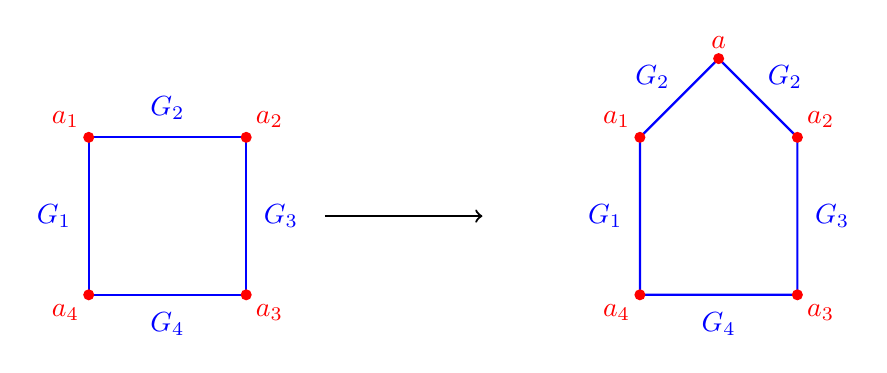
\begin{tikzpicture}
 
    % Left side (Square)
    % Define points for square
    \coordinate (a1) at (0, 0);
    \coordinate (a2) at (2, 0);
    \coordinate (a3) at (2, -2);
    \coordinate (a4) at (0, -2);

    % Draw square with labels
    \draw[thick, blue] (a1) -- (a2) -- (a3) -- (a4) -- cycle;
    \fill[red] (a1) circle (2pt) node[above left] {$a_1$};
    \fill[red] (a2) circle (2pt) node[above right] {$a_2$};
    \fill[red] (a3) circle (2pt) node[below right] {$a_3$};
    \fill[red] (a4) circle (2pt) node[below left] {$a_4$};
    
    % Label edges
    \node[above, blue] at (1, 0.1) {$G_2$};
    \node[right, blue] at (2.1, -1) {$G_3$};
    \node[below, blue] at (1, -2.1) {$G_4$};
    \node[left, blue] at (-0.1, -1) {$G_1$};

    % Arrow between diagrams (shifted right)
    \draw[->, thick] (3, -1) -- (5, -1);

    % Right side (Pentagon, shifted right)
    % Define points for pentagon
    \coordinate (b1) at (7, 0);
    \coordinate (b2) at (9, 0);
    \coordinate (b3) at (9, -2);
    \coordinate (b4) at (7, -2);
    \coordinate (a) at (8, 1);  % New point at top

    % Draw pentagon with labels
    \draw[thick, blue] (b1) -- (a) -- (b2) -- (b3) -- (b4) -- cycle;
    \fill[red] (b1) circle (2pt) node[above left] {$a_1$};
    \fill[red] (b2) circle (2pt) node[above right] {$a_2$};
    \fill[red] (b3) circle (2pt) node[below right] {$a_3$};
    \fill[red] (b4) circle (2pt) node[below left] {$a_4$};
    \fill[red] (a) circle (2pt) node[above] {$a$};

    % Label edges
    \node[above left, blue] at (7.5, 0.5) {$G_2$};
    \node[above right, blue] at (8.5, 0.5) {$G_2$};
    \node[right, blue] at (9.1, -1) {$G_3$};
    \node[below, blue] at (8, -2.1) {$G_4$};
    \node[left, blue] at (6.9, -1) {$G_1$};  % New edge label for left side

      
   \end{tikzpicture}     
   \caption{Illustration of 
${\cal G}^{(a)}_{k}$ for $n=4$. Taken from \cite{YY_25}.}
        \label{fig:op_gka}
 \end{figure}

 \noindent 
 \emph{2.}  For $1 \le k < l \le n$, we define a ``left" cut-and-glue operator ${\cal G}^{(a), L}_{k, l}$. Let ${\cal G}^{(a), L}_{k, l} \circ {\cal L}_{t, \boldsymbol{\sigma}, \textbf{a}}$ be the following loop. Cut the $k$-th and $l$-th edges $G_t(\sigma_k)$ and $G_t(\sigma_l)$ (creating four end points and two ``chains"). Glue the two new ends of the chain that contains $E_{a_n}$ and insert a new $E_a$ at the gluing point.
    
    \begin{figure}[ht]
        \centering
         \scalebox{0.8}{
       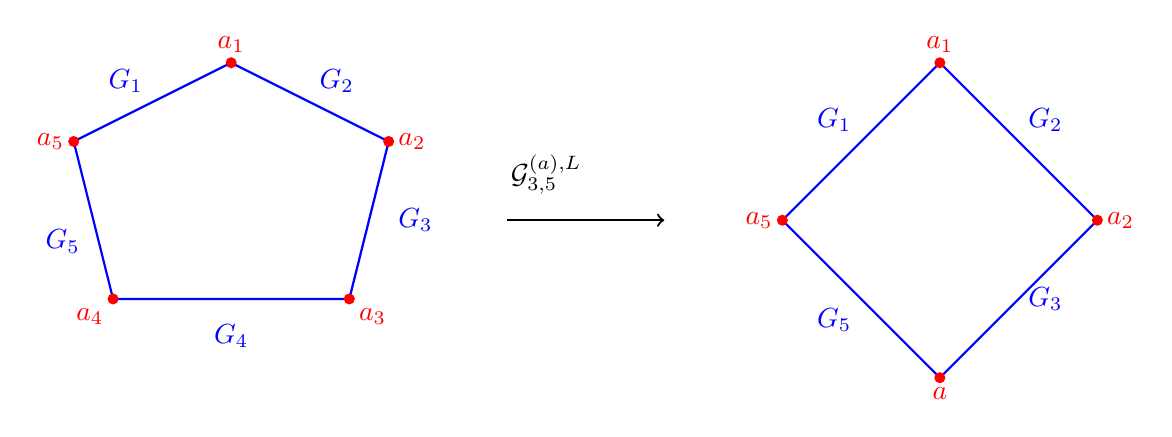
\begin{tikzpicture}
        % Left side (Pentagon)
        % Define points for pentagon
        \coordinate (a1) at (0, 2);
        \coordinate (a2) at (2, 1);
        \coordinate (a3) at (1.5, -1);
        \coordinate (a4) at (-1.5, -1);
        \coordinate (a5) at (-2, 1);

        % Draw pentagon with labels
        \draw[thick, blue] (a1) -- (a2) -- (a3) -- (a4) -- (a5) -- cycle;
        \fill[red] (a1) circle (2pt) node[above] {$a_1$};
        \fill[red] (a2) circle (2pt) node[right] {$a_2$};
        \fill[red] (a3) circle (2pt) node[below right] {$a_3$};
        \fill[red] (a4) circle (2pt) node[below left] {$a_4$};
        \fill[red] (a5) circle (2pt) node[left] {$a_5$};

        % Label edges
        \node[above right, blue] at (1, 1.5) {$G_2$};
        \node[right, blue] at (2, 0) {$G_3$};
        \node[below, blue] at (0, -1.2) {$G_4$};
        \node[below left, blue] at (-1.8, 0) {$G_5$};
        \node[above left, blue] at (-1, 1.5) {$G_1$};

        % Arrow between diagrams
        \draw[->, thick] (3.5, 0) -- (5.5, 0);
        \node[above] at (4, 0.2) {$ {\cal G}^{(a),L}_{3,5}$};

        % Right side (Diamond shape with four points)
        % Define points for diamond shape
        \coordinate (b1) at (9, 2);     % Top
        \coordinate (b2) at (11, 0);     % Right
        \coordinate (a) at (9, -2);     % Bottom (new point a)
        \coordinate (b5) at (7, 0);     % Left

        % Draw diamond shape
        \draw[thick, blue] (b1) -- (b2) -- (a) -- (b5) -- cycle;
        
        % Fill and label points
        \fill[red] (b1) circle (2pt) node[above] {$a_1$};
        \fill[red] (b2) circle (2pt) node[right] {$a_2$};
        \fill[red] (a) circle (2pt) node[below] {$a$};
        \fill[red] (b5) circle (2pt) node[left] {$a_5$};

        % Label edges
        \node[above right, blue] at (10, 1) {$G_2$};
        \node[right, blue] at (10, -1) {$G_3$};
        \node[below left, blue] at (8, -1) {$G_5$};
        \node[above left, blue] at (8, 1) {$G_1$};
    \end{tikzpicture}
    }
        \caption{Illustration of operator ${\cal G}^{(a), L}_{k, l}$. Taken from \cite{YY_25}.}
        \label{fig:op_gLeft}
    \end{figure}

  \noindent 
 \emph{3.}  For $1 \le k < l \le n$, we define a ``right" cut-and-glue operator ${\cal G}^{(a), R}_{k, l}$ the same way, but we instead glue the two new ends of the chain that does not contain $E_{a_n}$. The length of the new loop is $l - k + 1$.
     \begin{figure}[ht]
        \centering
       \scalebox{0.8}{  % Scale down to 80%
    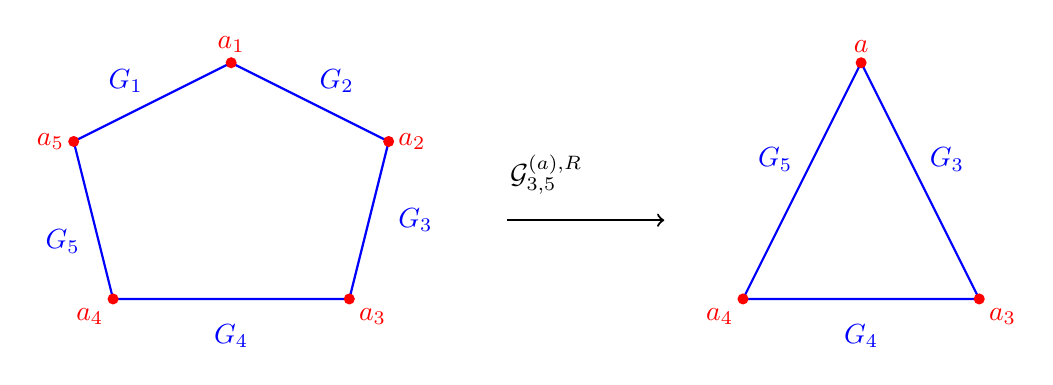
\begin{tikzpicture}
        % Left side (Pentagon)
        % Define points for pentagon
        \coordinate (a1) at (0, 2);
        \coordinate (a2) at (2, 1);
        \coordinate (a3) at (1.5, -1);
        \coordinate (a4) at (-1.5, -1);
        \coordinate (a5) at (-2, 1);

        % Draw pentagon with labels
        \draw[thick, blue] (a1) -- (a2) -- (a3) -- (a4) -- (a5) -- cycle;
        \fill[red] (a1) circle (2pt) node[above] {$a_1$};
        \fill[red] (a2) circle (2pt) node[right] {$a_2$};
        \fill[red] (a3) circle (2pt) node[below right] {$a_3$};
        \fill[red] (a4) circle (2pt) node[below left] {$a_4$};
        \fill[red] (a5) circle (2pt) node[left] {$a_5$};

        % Label edges
        \node[above right, blue] at (1, 1.5) {$G_2$};
        \node[right, blue] at (2, 0) {$G_3$};
        \node[below, blue] at (0, -1.2) {$G_4$};
        \node[below left, blue] at (-1.8, 0) {$G_5$};
        \node[above left, blue] at (-1, 1.5) {$G_1$};

        % Arrow between diagrams
        \draw[->, thick] (3.5, 0) -- (5.5, 0);
        \node[above] at (4, 0.2) {${\cal G}^{(a),R}_{3,5}$};

        % Right side (Triangle)
        % Define points for triangle
        \coordinate (a) at (8, 2);      % Top point (a)
        \coordinate (a3) at (9.5, -1);  % Bottom right point (a3)
        \coordinate (a4) at (6.5, -1);  % Bottom left point (a4)

        % Draw triangle with labels
        \draw[thick, blue] (a) -- (a3) -- (a4) -- cycle;

        % Fill and label points
        \fill[red] (a) circle (2pt) node[above] {$a$};
        \fill[red] (a3) circle (2pt) node[below right] {$a_3$};
        \fill[red] (a4) circle (2pt) node[below left] {$a_4$};

        % Label edges
        \node[above right, blue] at (8.75, 0.5) {$G_3$};
        \node[below, blue] at (8, -1.2) {$G_4$};
        \node[above left, blue] at (7.25, 0.5) {$G_5$};

    \end{tikzpicture}
    }  % End of scalebox
         \caption{Illustration of operator ${\cal G}^{(a), R}_{k, l}$. Taken from \cite{YY_25}.}
        \label{fig:op_gRight}
    \end{figure}  
\end{definition}


 
 The following result gives the evolution for a loop along the flow of $G^{(E)}_{t}$. It is derived via the It\^o formula. Throughout this paper, we let $\textbf{a}=(a_{1},\ldots,a_{n})$ be a vector of indices in $\Z_{L}^{2}$, and we let $a\in\Z_{L}^{2}$ be a single index that is separate from $\textbf{a}$. Finally, for convenience, we will use the notation $\partial_{(x,y)}:=\partial_{H_t(x,y)}$.
 
 
 
%
\begin{lemma}[The loop hierarchy] \label{lem:SE_basic}
We have the following ``loop hierarchy" SDE:
\begin{align}\label{eq:mainStoflow}
    d\mathcal{L}_{t, \boldsymbol{\sigma}, \textbf{a}} =& 
    \mathcal{E}^{(M)}_{t, \boldsymbol{\sigma}, \textbf{a}} 
    +
    \mathcal{E}^{(\widetilde{G})}_{t, \boldsymbol{\sigma}, \textbf{a}} 
    +
   W^{2}\cdot \sum_{1 \le k < l \le n} \sum_{a, b} \left( \mathcal{G}^{(a), L}_{k, l} \circ \mathcal{L}_{t, \boldsymbol{\sigma}, \textbf{a}} \right) S^{(B)}_{ab} \left( \mathcal{G}^{(b), R}_{k, l} \circ \mathcal{L}_{t, \boldsymbol{\sigma}, \textbf{a}} \right) dt. 
\end{align}
 Above, we used the notation 
  \begin{align} \label{def_Edif}
\mathcal{E}^{(M)}_{t, \boldsymbol{\sigma}, \textbf{a}} :  = & \sum_{\alpha=(x,y)} 
  \left( \partial_{  \alpha} \; {\cal L}_{t, \boldsymbol{\sigma}, \textbf{a}}  \right)
 \cdot \left(S _\alpha\right)^{1/2} \cdot
  \mathrm{d} \left({B}_t\right)_{\alpha} \\\label{def_EwtG}
  \mathcal{E}^{(\widetilde{G})}_{t, \boldsymbol{\sigma}, \textbf{a}}: = &   W^{2}\cdot \sum_{1 \le k \le n} \sum_{a, b} \; 
 \left \langle \widetilde{G}_t(\sigma_k) E_a \right\rangle
  \cdot S^{(B)}_{ab} \cdot
  \left( {\cal G}^{(b)}_{k} \circ {\cal L}_{t, \boldsymbol{\sigma}, \textbf{a}} \right) dt ,\quad \quad \widetilde{G}_t = G_t - m.
\end{align}
  \end{lemma}
  
The factor of $W^{2}$ in ${\cal E}^{(\widetilde{G})}$ comes from the normalization that $E_{a}$ has a factor of $W^{-2}$. In order to solve this hierarchy of SDEs, we introduce the notion of a convolution tree ${\cal K}$.

\begin{definition}\label{Def_Ktza}
For 
$$
\boldsymbol{\sigma}=(\sigma_1, \sigma_2, \cdots \sigma_n),\quad 
\boldsymbol{a}=(a_1, a_2, \cdots a_n)
,\quad \sigma_i \in \{+,-\}, \quad
a_i\in \mathbb Z_L^{2}, \quad 1\le i\le n
$$
and  $m(\sigma)$ defined in \eqref{def_mtzk}, we define  ${\cal K}_{t, \boldsymbol{\sigma}, \textbf{a}}$ to be the unique solution to the equation 
 \begin{align}\label{pro_dyncalK}
       \frac{d}{dt}\,{\cal K}_{t, \boldsymbol{\sigma}, \textbf{a}} 
       =  
       W^{2}\cdot  \sum_{1 \le k < l \le n} \sum_{a, b} \; \left( {\cal G}^{(a), L}_{k, l} \circ {\cal K}_{t, \boldsymbol{\sigma}, \textbf{a}} \right) S^{(B)}_{ab} \left( {\cal G}^{(b), R}_{k, l} \circ {\cal K}_{t, \boldsymbol{\sigma}, \textbf{a}} \right)  
    \end{align}
with initial data
$$
    {\cal K}_{0, \boldsymbol{\sigma}, \textbf{a}} =  {W^{-2(n-1)}} \cdot \prod_{k=1}^n m (\sigma_k) \cdot \textbf{1}(a_1 = a_2 = \cdots = a_n).
$$
Here, we define the ${\cal G}$ operator acting on ${\cal K}$ in the same way as it acts on ${\cal L}$,  i.e.,  
  \be\label{calGonIND}
     {\cal G}^{(a),\,L }_{k,l}  \circ {\cal K}_{t, \boldsymbol{\sigma}, \textbf{a}} = {\cal K}_{t, \; {\cal G}^{(a),\,L }_{k,l}  (\boldsymbol{\sigma}, \textbf{a})}  \quad \forall t, k, \boldsymbol{\sigma}, \textbf{a},   
       \ee
and similarly for  ${\cal G}^{(b),\, R }_{k,l}$. 
For the special case $n=1$, we define % the r.h.s. of \eqref{pro_dyncalK} is zero. Therefore for $n=1$ case
$
{\cal K}_{t,\,+,\, a}=m$ and  ${\cal K}_{t,\,-,\, a}=\overline m$ for $0\le t\le 1$. 
\end{definition}

Note that the lengths of ${\cal G}^{(a), L}_{k, l} \circ {\cal K}_{t, \boldsymbol{\sigma}, \textbf{a}}$ and ${\cal G}^{(a), R}_{k, l} \circ {\cal K}_{t, \boldsymbol{\sigma}, \textbf{a}}$ are no greater than the  length of ${\cal K}_{t, \boldsymbol{\sigma}, \textbf{a}}$. Thus, 
the system of equations for $\cal K$ can be solved inductively in the length of ${\cal K}$; we illustrate this in the next section.

\subsection{The propagator \texorpdfstring{$\Theta_\xi^{(B)}$}{Theta} and an estimate on \texorpdfstring{${\cal K}$}{ K}}
 
The key object that we need to analyze ${\cal K}$ is the following propagator.
 
 \begin{definition}\label{def_Theta}
We define the propagator $\Theta^{(B)}_{\xi}$ to be the following $L^{2}\times L^{2}$ matrix:
\begin{equation}\label{def_Thxi}
    \Theta^{(B)}_\xi := \frac{1}{1 - \xi \cdot S^{(B)}}, \quad \xi \in \mathbb{C}, \quad |\xi| < 1.
\end{equation}
(The superscript $B$ indicates a block-level matrix, i.e. one whose indices are parameterized by $\Z_{L}^{2}$.)
\end{definition}

For convenience, we often omit the superscript $(B)$ . (We remind the readers that $\Theta$  was often  used to denote the \(N \times N\) matrix  \((1 - \xi S)^{-1}\) in the literature.   In this paper,  $\Theta_\xi= \Theta_\xi^{(B)}$.) We note that
\begin{equation}\label{deri_Thxi}
    \partial_\xi \Theta^{(B)}_\xi = \Theta^{(B)}_\xi \cdot S^{(B)} \cdot \Theta^{(B)}_\xi.
\end{equation}

The following  three special  cases are often used in this paper (note that $|m|=|m^{(E)}|=1$ in our setting):
\[
\Theta^{(B)}_{t m^2}, \quad \Theta^{(B)}_{t \bar{m}^2}, \quad \text{and} \quad \Theta^{(B)}_{t |m|^2} = \Theta^{(B)}_{t}.
\]



We now collect the following important properties of $\Theta^{(B)}$. 
\begin{lemma}\label{lem_propTH}
Suppose that  $\xi\in \mathbb C$ satisfies $|\xi|< 1$.  Define
$$
 \hat{\ell}(\xi) := \min\left((|1-\xi|)^{-1/2},\; L\right),\quad \xi\in \mathbb C 
$$
Then  $\Theta^{(B)}_\xi$ has the following properties:
\begin{enumerate}
    \item Symmetry: $ (\Theta^{(B)}_{\xi})_{ab}= (\Theta^{(B)}_{\xi})_{ba}$.
    \item Translation invariance: $
    (\Theta^{(B)}_{\xi})_{ab}= (\Theta^{(B)}_{\xi})_{a+s, b+s}$ for any $s \in \mathbb{Z}_L^2$.
    \item Commutativity: $\left[S^{(B)}, \Theta^{(B)}_{\xi}\right]=\left[\Theta^{(B)}_{\xi\,'}, \Theta^{(B)}_{\xi}\right]=0$ for all $\xi,\xi'$.
    \item For any $ 0 \le \xi < 1$, we have the random walk representation $\Theta_\xi^{(B)}=\sum_{k=0}^{\infty}\;  \xi^k \cdot (S^{(B)})^k$.
     \item Exponential decay at length scale $\hat \ell(\xi) $ for $\xi\in\{tm^{2},t\overline{m}^{2},t|m|^{2}\}$: 
     \begin{equation}\label{prop:ThfadC}     (\Theta^{(B)}_{\xi})_{ab}\prec \frac{e^{-c\cdot|a-b|_{L}\big/ \hat{\ell}(\xi)}}{|1-\xi|\cdot [\hat \ell (\xi)]^{2}}.  
     \end{equation}     
     \item Derivative bounds for $\xi\in\{tm^{2},t\overline{m}^{2},t|m|^{2}\}$: for any $s \in \mathbb{Z}_L^2$, we have 
     \begin{equation}\label{prop:BD1}     
    \left| (\Theta^{(B)}_{\xi})_{ab}-(\Theta^{(B)}_{\xi})_{a(b+s)}\right|\prec \frac{|s|_L}{{|a-b|_{L}+1}}{+\frac{|s|_{L}}{[\hat{\ell}(\xi)]^{2}|1-\xi|^{1/2}}}   
     \end{equation}
     \begin{equation}\label{prop:BD2}     
     \left|2 (\Theta^{(B)}_{\xi})_{ab}-(\Theta^{(B)}_{\xi})_{a(b+s)}-(\Theta^{(B)}_{\xi})_{a(b-s)}\right|\prec  \frac{|s|_L^2}{|a-b|_L^{2}+1 }+{\frac{|s|_{L}^{2}}{[\hat{\ell}(\xi)]^{2}}} . 
     \end{equation}

\end{enumerate}
\end{lemma}
{The proof of Lemma \ref{lem_propTH} is based on Fourier analysis on $\Z_{L}^{2}$: a contour shift in the momentum variable yields the exponential decay, and a dyadic decomposition of the momenta yields the derivative bounds. A proof is given in Section \ref{sec_TH}; the argument is elementary, so we give an intuitive explanation of Lemma \ref{lem_propTH} below.

The first four properties in Lemma \ref{lem_propTH} are standard. The exponential decay \eqref{prop:ThfadC} for the discrete Laplacian on $\Z^{2}$ (instead of $S^{(B)}-\mathrm{Id}$) can be found in Theorem 1.3 of \cite{MS22} (see also the discussion following it therein). The difference between the full space $\Z^{2}$ and the torus $\Z_{L}^{2}$ is that if $\hat{\ell}(\xi)=L$, so that $|1-\xi|^{-1/2}\geq L$, then the periodic boundary conditions on $\Z_{L}^{2}$ automatically introduce a space-cutoff of scale $L$ (before the cutoff at scale $|1-\xi|^{-1/2}$ that is imposed by the resolvent). One can also check that \eqref{prop:ThfadC} implies 
%
\begin{align*}
\sum_{b\in\Z_{L}^{2}}(\Theta^{(B)}_{\xi})_{ab}\prec|1-\xi|^{-1},
\end{align*}
%
which can be checked using the random walk representation as well. 

The gradient bounds \eqref{prop:BD1}-\eqref{prop:BD2} are standard, in that the Green's function for the Laplacian on $\R^{2}$ is $\log|x|$. Thus, the first terms on the right-hand side of \eqref{prop:BD1}-\eqref{prop:BD2} agree with its derivatives. (The support-length of the gradients is also of order $\hat{\ell}(\xi)$, but we will not need this fact.) The additional corrections come from the periodic boundary of $\Z_{L}^{2}$. The scaling of the last term in \eqref{prop:BD2} agrees with the heuristic that $\Theta^{(B)}$ is the resolvent for the diffusion of a generator, so its second-derivative should have $L^{1}$ norm of size $\mathrm{O}_{\prec}(1)$. The last term in \eqref{prop:BD1} therefore interpolates between \eqref{prop:ThfadC} and the last term in \eqref{prop:BD2}.}


Let us now illustrate ${\cal K}_{t,\boldsymbol{\sigma},(a_{1},a_{2})}$ for $n=2$. In this case, the defining convolution tree equation  \eqref{pro_dyncalK} is 
\begin{align}
    \frac{d}{dt}\, \mathcal{K}_{t, \boldsymbol{\sigma}, (a_1, a_2)} = W^{2} \cdot \sum_{a, b} \mathcal{K}_{t, \boldsymbol{\sigma}, (a_1, a)} \cdot S^{(B)}_{ab} \cdot \mathcal{K}_{t, \boldsymbol{\sigma}, (b, a_2)}
\end{align}
Throughout this paper, we will often use the following convenient notation: 
\begin{equation}\label{eq_defm_i}
    m_i = m(\sigma_i).
\end{equation}
Using the propagator  $\Theta^{(B)}$ in \eqref{def_Thxi} and, \eqref{deri_Thxi}, a short calculation yields
\begin{equation}\label{Kn2sol}
    \mathcal{K}_{t, \boldsymbol{\sigma}, \textbf{a}} = W^{-2} m_1 m_2 \left(\Theta^{(B)}_{t \cdot m_1 m_2}\right)_{a_1 a_2}, \quad \textbf{a} = (a_1, a_2)
\end{equation}
%Now for $2$-$G$-loop, the definition of $\cal K$ in Def. \ref{Def_Ktza} shows (here we dropped the superscript ${(E)}$), 
In particular, if we consider the two cases $\boldsymbol{\sigma}=(+,-)$ and $\boldsymbol{\sigma}=(+,+)$, then
\begin{equation}\label{Kn2sol2}
{\cal K}_{t,\boldsymbol{\sigma},(a,b)}
=   W^{-2} \cdot \begin{cases}
     |m |^2\left[\left(1- {  t }|m |^2 S^{(B)}\right)^{-1}\right]_{ab} &, \quad \boldsymbol{\sigma}=(+,-)\\
  m^2\left[\left(1- {  t } m^2 S^{(B)}\right)^{-1}\right]_{ab}  &, \quad \boldsymbol{\sigma}=(+,+)    
\end{cases}
\end{equation}

In the case where $n=3$, we have the following formula (which comes from Example 2.16 in \cite{YY_25} and comes directly from the convolution tree equation, hence it has no dimension dependence):
$$
{\cal K}_{t, \boldsymbol{\sigma}, \textbf{a}} = \sum_{b_1 b_2 b_3} \left(\Theta^{(B)}_{t \cdot m_1 m_2}\right)_{a_1 b_1} \left(\Theta^{(B)}_{t \cdot m_2 m_3}\right)_{a_2 b_2} \left(\Theta^{(B)}_{t \cdot m_3 m_1}\right)_{a_3 b_3} \cdot {\cal K}_{0, \boldsymbol{\sigma}, \textbf{b}}, \quad \textbf{b} = (b_1, b_2, b_3).
$$

\begin{lemma}\label{ML:Kbound}
Recall $\hat \ell $ in \eqref{prop:ThfadC}. We have
\begin{equation}\label{eq:bcal_k}
  {\cal K}_{t, \boldsymbol{\sigma}, \textbf{a}}  \prec M_{t}^{-n+1},\quad  \ell_t :  =\hat\ell(t)= \min\left((|1-t|)^{-1/2},\; L\right), \quad M_{t}:=W^{2}\ell_{t}^{2}\eta_{t}.     
\end{equation}
\end{lemma}

Finally, we note that for any fixed \(|E| < 2 - \kappa\), we have $\im z_t = \im z_t^{(E)} = \im m^{(E)} \cdot (1 - t) \sim (1 - t)$. Thus, \(\ell(z)\) from \eqref{def_ellz} and \(\ell_t\) from \eqref{eq:bcal_k} are the same order, in that $\ell(z_t) \sim \ell_t = \hat{\ell}(t)$. Furthermore, for \(z\), \(t\), and \(E\) satisfying \eqref{eq:zztE} and \eqref{eq:zztE2}, we have $\im z\sim \im z^{(E)}_t$ and $\ell(z) \sim \ell(z^{(E)}_t) \sim \ell_t$. Since these terms are the same order, in the following, we will use only \(\ell_t\).
 





\subsection{Estimates on loops}
 

Our main estimates for the  $G$-loop  are given below. (Recall $\prec$ in Definition \ref{stoch_domination}, and recall $\ell_{t},M_{t}$ in \eqref{eq:bcal_k}.) 

\begin{lemma}\label{ML:GLoop}
%Denote the length scale $\ell_t:=\ell(z_t)$.  
For any $\kappa, \tau>0$ and  
$E \in[-2+\kappa, 2-\kappa], \, 0\le t\le 1-N^{-1+\tau}$,  
we have 
\begin{equation}\label{Eq:L-KGt}
 \max_{\boldsymbol{\sigma}, \textbf{a}}\left|{\cal L}_{t, \boldsymbol{\sigma}, \textbf{a}}-{\cal K}_{t, \boldsymbol{\sigma}, \textbf{a}}\right|\prec M_{t}^{-n},\quad \eta_t:=\im z_t,  %\quad \ell_t:=\ell(z_t)
\end{equation}
 \begin{equation}\label{Eq:L-KGt2}
\max_{\boldsymbol{\sigma}, \textbf{a}}\left|{\cal L}_{t, \boldsymbol{\sigma}, \textbf{a}} \right|\prec M_{t}^{-n+1}. %\quad \eta_t:=\im z_t,\quad \ell_t:=\ell(z_t)
\end{equation}
\end{lemma}
\begin{lemma}[$2$-loop estimate]\label{ML:GLoop_expec}
With the notations and assumptions of the previous lemma, if $\boldsymbol{\sigma}=(+,-)$ and $ \textbf{a}=(a_1, a_2)$, then
we have
\begin{equation}\label{Eq:Gdecay}
 \left| {\cal L}_{t, \boldsymbol{\sigma}, \textbf{a}}-{\cal K}_{t, \boldsymbol{\sigma}, \textbf{a}}\right|\prec M_{t}^{-2}\exp \left(-\frac{|a_1-a_2|_{L}^{1/2} }{\ell_t^{1/2}}\right)+W^{-D}. 
\end{equation}
\end{lemma}


\begin{lemma}[Local law for $G_t$]\label{ML:GtLocal}
   With the notations and assumptions of the previous lemma, we have 
\begin{equation}\label{Gt_bound}
 \|G^{(E)}_{t,+}-m^{(E)}\|_{\max}\prec M_{t}^{-1/2}.
   \end{equation} 
\end{lemma}
 


\begin{lemma}[Improved expectation bound on $2$-loop]\label{ML:exp}
Adopt the notations and assumptions of the previous lemma. Fix any $\boldsymbol{\sigma}\in\{+,-\}^{2}$ and $\textbf{a}=(a_{1},a_{2})\in\Z_{L}^{2}\times\Z_{L}^{2}$. We have 
%
\begin{align}
|\E{\cal L}_{t,\boldsymbol{\sigma},\textbf{a}}-{\cal K}_{t,\boldsymbol{\sigma},\textbf{a}}|\prec M_{t}^{-3}.\label{eq:step6main}
\end{align}
%
\end{lemma}







\medskip 

\begin{proof}[Proof of Theorems \ref{MR:locSC} and \ref{MR:QDiff}]
This is the same argument as the proof of Theorems 2.3 and 2.5 in \cite{YY_25}. For each $z$ in Theorems \ref{MR:locSC} and \ref{MR:QDiff}, Lemma \ref{zztE} gives $E$ and $t$ satisfying \eqref{eq:zztE}, \eqref{eq:zztE2}, and
$$
(1-t) \sim \im z_t \sim \im z \geq N^{-1+\tau}, \quad \eta_t \sim \eta, \quad \ell_t \sim \ell(z).
$$
Combining \eqref{mtEmz} and \eqref{GtEGz} gives
\begin{equation}\label{Gmt1/2Gm}
G(z) - m_{sc}(z) = t^{1/2} \left(G_t^{(E)} - m^{(E)}\right).
\end{equation}
Thus, \eqref{G_bound} follows from the estimate \eqref{Gt_bound} on $G_t - m$. Similarly, the partial tracial local law \eqref{G_bound_ave} follows from \eqref{Eq:L-KGt} for $n=1$ and the definition ${\cal K}_{t,+,a}=m^{(E)}$ from Definition \ref{Def_Ktza}. Next, by Definition \ref{Def:G_loop},
\begin{equation}\label{Gmt1/2Gm2}
\tr GE_aGE_b = t \cdot {\cal L}_{t, (+,+),(a,b)}, \quad \tr GE_aG^\dagger E_b = t \cdot {\cal L}_{t, (+,-),(a,b)}.
\end{equation}
By using the formula \eqref{Kn2sol} and recalling from \eqref{mtEmz} that $m_{sc}(z)=t^{1/2}m^{(E)}$, we get
$$
t \cdot {\cal K}_{t, (+,+),(a,b)} = W^{-2} m^2_{sc}(z) \cdot \left[\frac{1}{1 - m^2_{sc}(z) \cdot S^{(B)}}\right]_{ab}, \quad t \cdot {\cal K}_{t, (+,-),(a,b)} = W^{-2} |m_{sc}(z)|^2 \cdot \left[\frac{1}{1 - |m_{sc}(z)|^2 \cdot S^{(B)}}\right]_{ab}.
$$
Therefore, \eqref{Meq:QdW1} and \eqref{Meq:QdW2} in Theorem \ref{MR:QDiff} follow from \eqref{Eq:L-KGt} in the case $n=2$. Finally, \eqref{Meq:QdS1}-\eqref{Meq:QdS2} follow from Lemma \ref{ML:exp}.
 \end{proof}




\bigskip

\subsection{Strategy of the proofs of main lemmas}

It turns out that Lemma \ref{ML:exp} will follow from Lemmas \ref{ML:GLoop}, \ref{ML:GLoop_expec}, and \ref{ML:GtLocal}. Thus, let us outline the proofs of Lemmas \ref{ML:GLoop}, \ref{ML:GLoop_expec} and \ref{ML:GtLocal}. The general strategy is the same as in Section 2 of \cite{YY_25}.
By Definitions \ref{Def:G_loop} and \ref{Def_Ktza}, we have
$$
G_{0}(+)=m\cdot I_{N\times N}, \quad {\cal L}_{0, \boldsymbol{\sigma},\textbf{a}}= {\cal K}_{0, \boldsymbol{\sigma},\textbf{a}},\quad \forall \; \boldsymbol{\sigma},\textbf{a}, 
$$
where $I_{N\times N}$ is the identity matrix. By construction, we know that:
\begin{align}\label{ini)bigasya}
    \hbox{    Lemmas \ref{ML:GLoop}, \ref{ML:GLoop_expec} and \ref{ML:GtLocal} hold at  $t=0$ with no error.}
\end{align}
The following result propagates the desired estimates forwards in time.


\begin{theorem}\label{lem:main_ind} Assume for some fixed $E$: $|E|\le 2-\kappa$ and $s\in [0,1]$ that Lemmas \ref{ML:GLoop}, \ref{ML:GLoop_expec}  and \ref{ML:GtLocal} hold at time $s$. That is, assume that %with $\eta_s:=\im z_s,\quad \ell_s:=\ell(z_s)$,   
for $1 \le n\in \mathbb N$ and large $D>0$, we have
\begin{align}\label{Eq:L-KGt+IND}
 \max_{\boldsymbol{\sigma}, \textbf{a}}\left|{\cal L}_{s, \boldsymbol{\sigma}, \textbf{a}}-{\cal K}_{s, \boldsymbol{\sigma}, \textbf{a}}\right|&\prec M_{s}^{-n}  
\\\label{Eq:Gdecay+IND}
 \left| {\cal L}_{s, \boldsymbol{\sigma}, \textbf{a}}-{\cal K}_{s, \boldsymbol{\sigma}, \textbf{a}}\right|&\prec M_{s}^{-2}\exp \left(- \frac{ |a_1-a_2|_{L}^{1/2} }{\ell_s^{1/2}}\right)+W^{-D} , \quad \boldsymbol{\sigma}=(+,-)
\\\label{Gt_bound+IND}
 \|G^{(E)}_{s ,+}-m^{(E)}\|_{\max} & \prec M_{s}^{-1/2}.
\end{align}
 Then for any $t>s$ satisfying $t\leq 1-N^{-1+\tau}$ for some fixed $\tau>0$ and
\begin{equation}\label{con_st_ind}
    M_{s}^{-1}\le \left(\frac{1-t}{1-s}\right)^{30}
\end{equation}
%Here $2024$ is just for a large number, the exact value will not affect our final results) then
we have 
\eqref{Eq:L-KGt+IND}, \eqref{Eq:Gdecay+IND} and \eqref{Gt_bound+IND} with $s$  replaced by $t$.   
\end{theorem}

\begin{proof}[Proof of Lemmas \ref{ML:GLoop}, \ref{ML:GLoop_expec},  and \ref{ML:GtLocal}]
For any $\tau$ and  $t \le 1-N^{-1+\tau}$,  choose $\tau'>0$ and $n_0 \in \mathbb N$ such that $M_{t}^{-1}\le  W^{- 30 \tau'}$ and $(1-t) = W^{-n_0 \tau'}$. We also choose a sequence of time-scales given by $1-s_{k} = W^{-k \tau'}$ for $ k \le n_0$, where $n_{0}$ is chosen so that $ s_{n_0}=t$. Since  $M_{s}$ is decreasing in  $s\in [0,1]$, we have 
   $$
M_{s_{k}}^{-1}\le M_{t}^{-1}\le W^{- 30\tau'}
= \left(\frac{1-s_{k+1}}{1-s_{k}}\right)^{30}
$$
for all $k$ such that  $k+1\le n_0$. We can now apply Theorem \ref{lem:main_ind} for $s=s_{k}$ for each $k$ inductively. (We note that $n_{0}=O(1)$, so the number of implicit $W^{\tau}$ factors we pick up from the meaning of $\prec$ is still $W^{\tau'}$ for $\tau'>0$ small.) This gives all the estimates in Lemmas \ref{ML:GLoop}, \ref{ML:GLoop_expec},  and \ref{ML:GtLocal} except for \eqref{Eq:L-KGt2}, which follows from \eqref{Eq:L-KGt} combined with the deterministic ${\cal K}$ estimate from Lemma \ref{ML:Kbound}.
\end{proof}


 
 
Theorem \ref{lem:main_ind} and Lemma \ref{ML:exp} will be proved in six steps. Their proofs are given in Section \ref{Sec:Stoflo}. The first five of these steps are meant to show Theorem \ref{lem:main_ind}. So, throughout the first five of these steps, we assume that the conditions of Theorem \ref{lem:main_ind} are satisfied. Each step builds on the conclusions of the preceding steps.

On the other hand, the last of these steps is separate in the sense that it is not part of the propagation idea used in the proofs of Lemmas \ref{ML:GLoop}, \ref{ML:GLoop_expec},  and \ref{ML:GtLocal} above.


\medskip 
\noindent 
\textbf{Step 1}   (A priori loop bounds): We will first show the following loop estimate:
 \begin{equation}\label{lRB1}
   {\cal L}_{u,\boldsymbol{\sigma}, \textbf{a}}\prec (\ell_u/\ell_s)^{2(n-1)}\cdot 
   M_{u}^{-n+1},\quad  s\le u\le t.
\end{equation}
We will also show the following weaker version of \eqref{Gt_bound+IND}:
\begin{equation}\label{Gtmwc}
    \|G_u-m\|_{\max}\prec  M_{u}^{-1/4},\quad s\le u\le t .
\end{equation} 
 




 \bigskip
\noindent 
\textbf{Step 2}  (A priori $2$-loop decay): 
 Next, we show the following local law for $u\in [s,t]$: 
 \begin{equation}\label{Gt_bound_flow}
     \|G_u-m\|_{\max}\prec  M_{u}^{-1/2},\quad s\le u\le t.
\end{equation} 
Hence \eqref{Gt_bound+IND} in Theorem \ref{lem:main_ind} will follow.  
In addition,  for any  
 $\boldsymbol{\sigma}=(+,-)$,   $s\le u\le t$, and $D>0$, we show   
 \begin{equation}\label{Eq:Gdecay_w}
\left| {\cal L}_{u, \boldsymbol{\sigma}, \textbf{a}}-{\cal K}_{u, \boldsymbol{\sigma}, \textbf{a}}\right| \prec \left(\eta_s/\eta_u\right)^4\cdot M_{u}^{-2}\exp \left(- \frac{|a_1-a_2|_{L}^{1/2}}{\ell_u^{1/2}}\right)+W^{-D} . \quad 
\end{equation}
   \bigskip
 \noindent 
\textbf{Step 3}   (Sharp  loop  bounds): 
Next, we show the following \emph{sharp} estimate on loops:
\begin{equation}\label{Eq:LGxb}
\max_{\boldsymbol{\sigma}, \textbf{a}}\left| {\cal L}_{u, \boldsymbol{\sigma}, \textbf{a}} \right|
\prec 
M_{u}^{-n+1} ,\quad \quad s\le u\le t, \quad\forall\, n\in \mathbb N.
\end{equation}


 \bigskip
 \noindent 
\textbf{Step 4}  (A sharp  $\cal L - \cal K$  bound): 
We show a sharp bound on ${\cal L}_{t}-{\cal K}_{t}$, which gives \eqref{Eq:L-KGt+IND} in Theorem  \ref{lem:main_ind}:
\begin{equation}\label{Eq:L-KGt-flow}
 \max_{\boldsymbol{\sigma}, \textbf{a}}\left|{\cal L}_{u, \boldsymbol{\sigma}, \textbf{a}}-{\cal K}_{u, \boldsymbol{\sigma}, \textbf{a}}\right|\prec M_{u}^{-n},\quad \quad s\le u\le t, \quad \forall\, n\in \mathbb N.
\end{equation}



 \bigskip
 \noindent 
\textbf{Step 5}  (A sharp decay bound): For  $ \boldsymbol{\sigma}=(+,-)$, we show the following, which gives \eqref{Eq:Gdecay+IND} in Theorem  \ref{lem:main_ind}:
 \begin{equation}\label{Eq:Gdecay_flow}
\left| {\cal L}_{u, \boldsymbol{\sigma}, \textbf{a}}-{\cal K}_{u, \boldsymbol{\sigma}, \textbf{a}}\right| \prec   M_{u}^{-2}\exp \left(- \frac{|a_1-a_2|_{L}^{1/2}}{\ell_u^{1/2}}\right)+W^{-D}. 
\end{equation}



 \bigskip
 \noindent 
\textbf{Step 6}  (Showing Lemma \ref{ML:exp}): As we showed earlier, Theorem \ref{lem:main_ind} implies Lemmas \ref{ML:GLoop}, \ref{ML:GLoop_expec}, and \ref{ML:GtLocal}. We then use these results to prove Lemma \ref{ML:exp}.


 

 



 



\subsection{Notations}
Here we summarize  global notations used in this paper. 
\begin{itemize}
    \item $W$ is band width, and $L^{2}$ is the number of blocks, so that $N=W^{2}\cdot L^{2}$;
    throughout, $L\geq3$, which is needed for $S^{(B)}$ to be the five-point stochastic matrix
    and is harmless because every statement below is asymptotic in $L\to\infty$
    \item ${\cal I}^{(2)}_a$ is the $a$-th block, $[x]$ is the block containing $x$, and $E_a$ is the following matrix supported on ${\cal I}^{(2)}_a$: 
    $$
    x\in {\cal I}^{(2)}_{[x]}, \quad (E_a)_{xy}=\delta_{xy}\cdot W^{-2}\cdot {\bf 1}(x\in {\cal I}^{(2)}_a)$$
    \item The periodic distance on $\mathbb{Z}_L$ is denoted by $|\cdot|_L$ and the periodic $L^1$ distance on $\mathbb{Z}_L^2$ is defined for any $a = (a(1), a(2))\in\mathbb{Z}_L^2$ by
    $$
    |a| = |a|_L = |a(1)|_L + |a(2)|_L.
    $$
    
    \item The matrices $S\in \mathbb R^{N\times N}$, $S^{(B)}\in \mathbb R^{L^{2}\times L^{2}}$, $S_W\in \mathbb R^{W^{2}\times W^{2}}$ are all related to the variances of entries of the random matrix $H$, and $S= S^{(B)}\otimes S_{W}$.
\item In the stochastic flow, we typically omit the superscript $(E)$ for simplicity, so that
\[
z_t = z_t^{(E)}, \quad G_t := (\sqrt{t} H - z_t)^{-1}, \quad m = \lim_{\varepsilon \searrow 0} m_{sc}(E + i \varepsilon).
\]
Additionally, we use $G_t$ to mean $(H_t - z_t)^{-1}$, where $H_t$ has the same distribution as $\sqrt{t} H$. The context will make it clear which interpretation of $G_t$ is being used.
\item The length-scale $\ell_t$ is defined in \eqref{eq:bcal_k} as $\ell_t:=\hat \ell(t)=\min(|1-t|^{-1/2}, L)\sim\ell(z_{t})$.

    \item The notation $\cal L$ denotes $G$-loops, and $\cal K$ denotes its deterministic approximation (the ``convolution tree'').

    \item The matrix $\Theta_\xi = \Theta^{(B)}_{\xi}$ is given in Definition \ref{def_Theta}.

    
    \item The quantities $\Xi^{({\cal L})}$, $\Xi^{({\cal L-K})}$, $\Xi^{({\cal C})}$ are loops that are normalized to have heuristic size of order $1$:
    
    \begin{align}
\Xi^{({\cal L})}_{t, m}&:= \max_{\boldsymbol{\sigma}, \textbf{a}} 
\left|{\cal L}_{t, \boldsymbol{\sigma}, \textbf{a}} \right|\cdot M_{t}^{m-1} \cdot {\bf 1}(\sigma \in \{+,-\}^m),
\label{def:XiL} \\
\Xi^{({\cal L-K})}_{t, m}&:= \max_{\boldsymbol{\sigma}, \textbf{a}}
\left|{ ({\cal L-K})}_{t, \boldsymbol{\sigma}, \textbf{a}} \right|\cdot M_{t}^{m }\cdot {\bf 1}(\sigma \in \{+,-\}^m).
\nonumber
\end{align}
\item The operators $\varTheta_{t,\boldsymbol{\sigma}}$ and ${\cal U}_{s, t,\boldsymbol{\sigma}}$ in Definition \ref{DefTHUST} appear in an ``integrated loop hierarchy" (Lemma \ref{Sol_CalL}). 
\item  The \(\cal G\) operators, such as \({\cal G}^{(a)}_k\), \({\cal G}^{(a),\,L}_{k,l}\), and \({\cal G}^{(a),\,R}_{k,l}\), are in Definition \ref{Def:oper_loop}. These represent the cutting and gluing of loops in the loop hierarchy.
 
 
\item  The \(\cal E\) terms represent lower-order terms in the (integrated) loop hierarchy \eqref{eq:mainStoflow} and \eqref{int_K-LcalE}. Specifically, \({\cal E}^{(M)}\) and \({\cal E}^{(\widetilde{G})}\) are defined in \eqref{def_Edif} and \eqref{def_EwtG}, respectively. The term \(\mathcal{E}^{((\mathcal{L}-\mathcal{K}) \times (\mathcal{L}-\mathcal{K}))}\) is defined in \eqref{def_ELKLK}. Additionally, \(\left( \mathcal{E} \otimes \mathcal{E} \right)\) and \(\left( \mathcal{E} \otimes \mathcal{E} \right)^{(k)}\) are defined in Definition \ref{def:CALE}.

\item  The quantity \({\cal T}^{(\cal L-\cal K)}_{t}\) is defined in \eqref{def_WTu}; it captures tail behavior of ${\cal L}-{\cal K}$. The quantity \({\cal T}_{t,D}\) represents a deterministic rough tail function, as defined in \eqref{def_WTuD}. 
\item The terms \({\cal J}_{u,D}\) and \(\cal J^*\) are introduced in \eqref{def_Ju} and \eqref{shoellJJ}, respectively, to describe the ratio between \({\cal T}^{(\cal L-\cal K)}_{t}\) and \({\cal T}_{t,D}\).

\item We often use an augmented length-scale $\ell_t^*=(\log W)^{3/2}\ell_t$. At this scale, $\Theta_t$ is exponentially small in $W$, but ${\cal T}_t$ is not. 
 

\end{itemize}
